\chapter{Results} \label{chap:Results}

\section{Introduction} \label{sec:intro_Results}

% Introduction to the chapter

\subsection{Parametric study on the analytical model} \label{subsec:parametricStudy_Results} 
In the present subsection, the variation of the beam properties for different parameter values will be shown. The beam geometry will be characterized through the cross-sectional aspect ratio $B/H$, the thickness ratio $t_2/t_1$ and the slenderness ratio $L/B$. The effect of these parameters on the sectional properties, twist and bending stiffness, and flexural and twisting compliance will be shown. Additionally, the variance of the stiffness ratio $E_1/E_2$ will also be included in the analysis.

\subsubsection{Results} \label{subsubsec:results_parametricStudy}

The influence of the cross-sectional aspect ratio $B/H$ on the torsional stiffness $G I_t$, the shear centre position $y_{\mathrm{SC}}$ and the flexural stiffness $E I_y$ is shown in Figures \ref{fig:GIt-E1overE2-BoverH}, \ref{fig:SC-E1overE2-BoverH} and \ref{fig:EIy-E1overE2-BoverH}, respectively. On its side, the effect of thickness ratio $t_2/t_1$ on the same three beam parameters is shown in Figures \ref{fig:GIt-E1overE2-t2overt1}, \ref{fig:SC-E1overE2-t2overt1} and \ref{fig:EIy-E1overE2-t2overt1}.

Additionally, the effect of the cross-sectional aspect ratio $B/H$ on the deflection and torsional compliance is shown on Figures \ref{fig:woverQ-E1overE2-BoverH} and \ref{fig:phioverQ-E1overE2-BoverH}, respectively. The corresponding plots when analysing the effect of the thickness ratio $t_2/t_1$ on the deflection and torsional compliance are shown on Figures \ref{fig:woverQ-E1overE2-t2overt1} and \ref{fig:phioverQ-E1overE2-t2overt1}, respectively. The beam's torsional compliance will be expressed as fraction of the twist at the tip divided by the vertical force applied, that is $|\phi_{\mathrm{tip}}| / Q$, while the beam deflection compliance will be expressed as fraction of the maximum vertical displacement at the tip divided by the vertical force applied, that is $w_{\mathrm{0,tip}} / Q$.

The effect of the slenderness ratio $L/B$ on the deflection and torsional compliances is shown in Figures \ref{fig:woverQ-E1overE2-LoverB} and \ref{fig:phioverQ-E1overE2-LoverB}, respectively.

%Figures variation of B/H
\begin{figure}[!htpb] %G I_t versus B/H
  \centering
  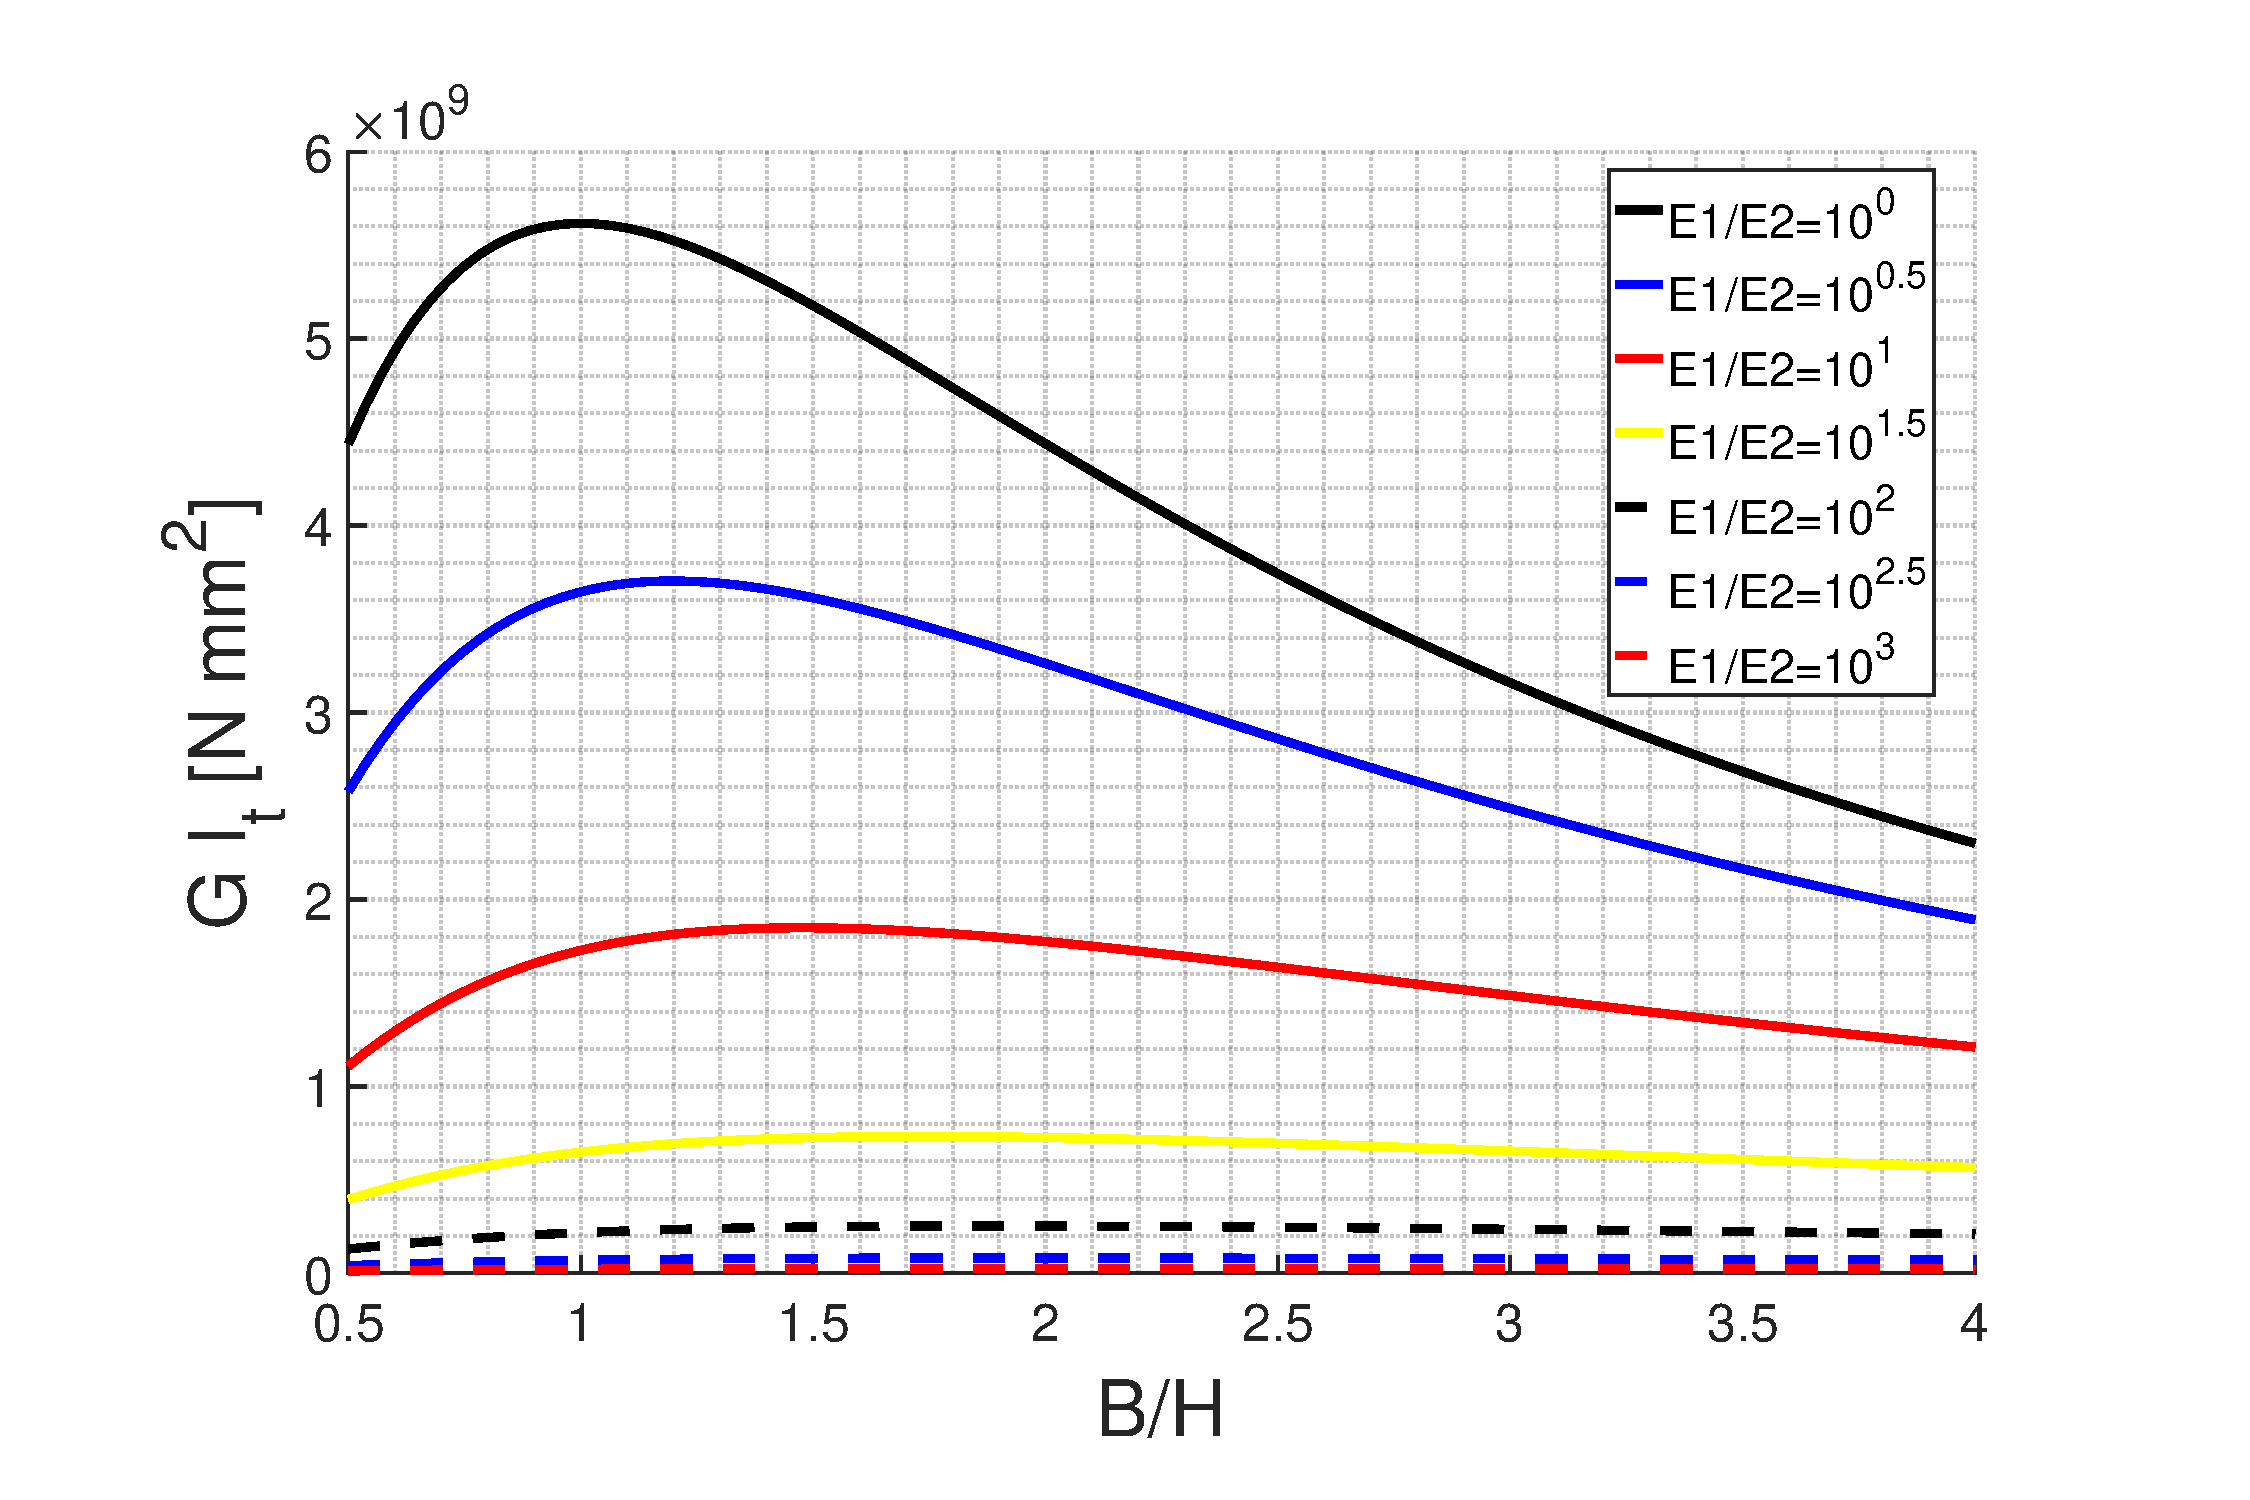
\includegraphics[width=0.8 \textwidth]{../../analytical/figures/GIt-E1overE2-BoverH}
  \caption[Influence of the cross-sectional aspect ratio $B/H$ on the torsional stiffness $GI_t$]{Influence of the cross-sectional aspect ratio $B/H$ on the torsional stiffness $GI_t$ is shown for various values of the stiffness ratio $E_1/E_2$ ranging from $10^0$ to $10^3$. }\label{fig:GIt-E1overE2-BoverH}
\end{figure}

\begin{figure}[!htpb] %Shear centre versus B/H
  \centering
  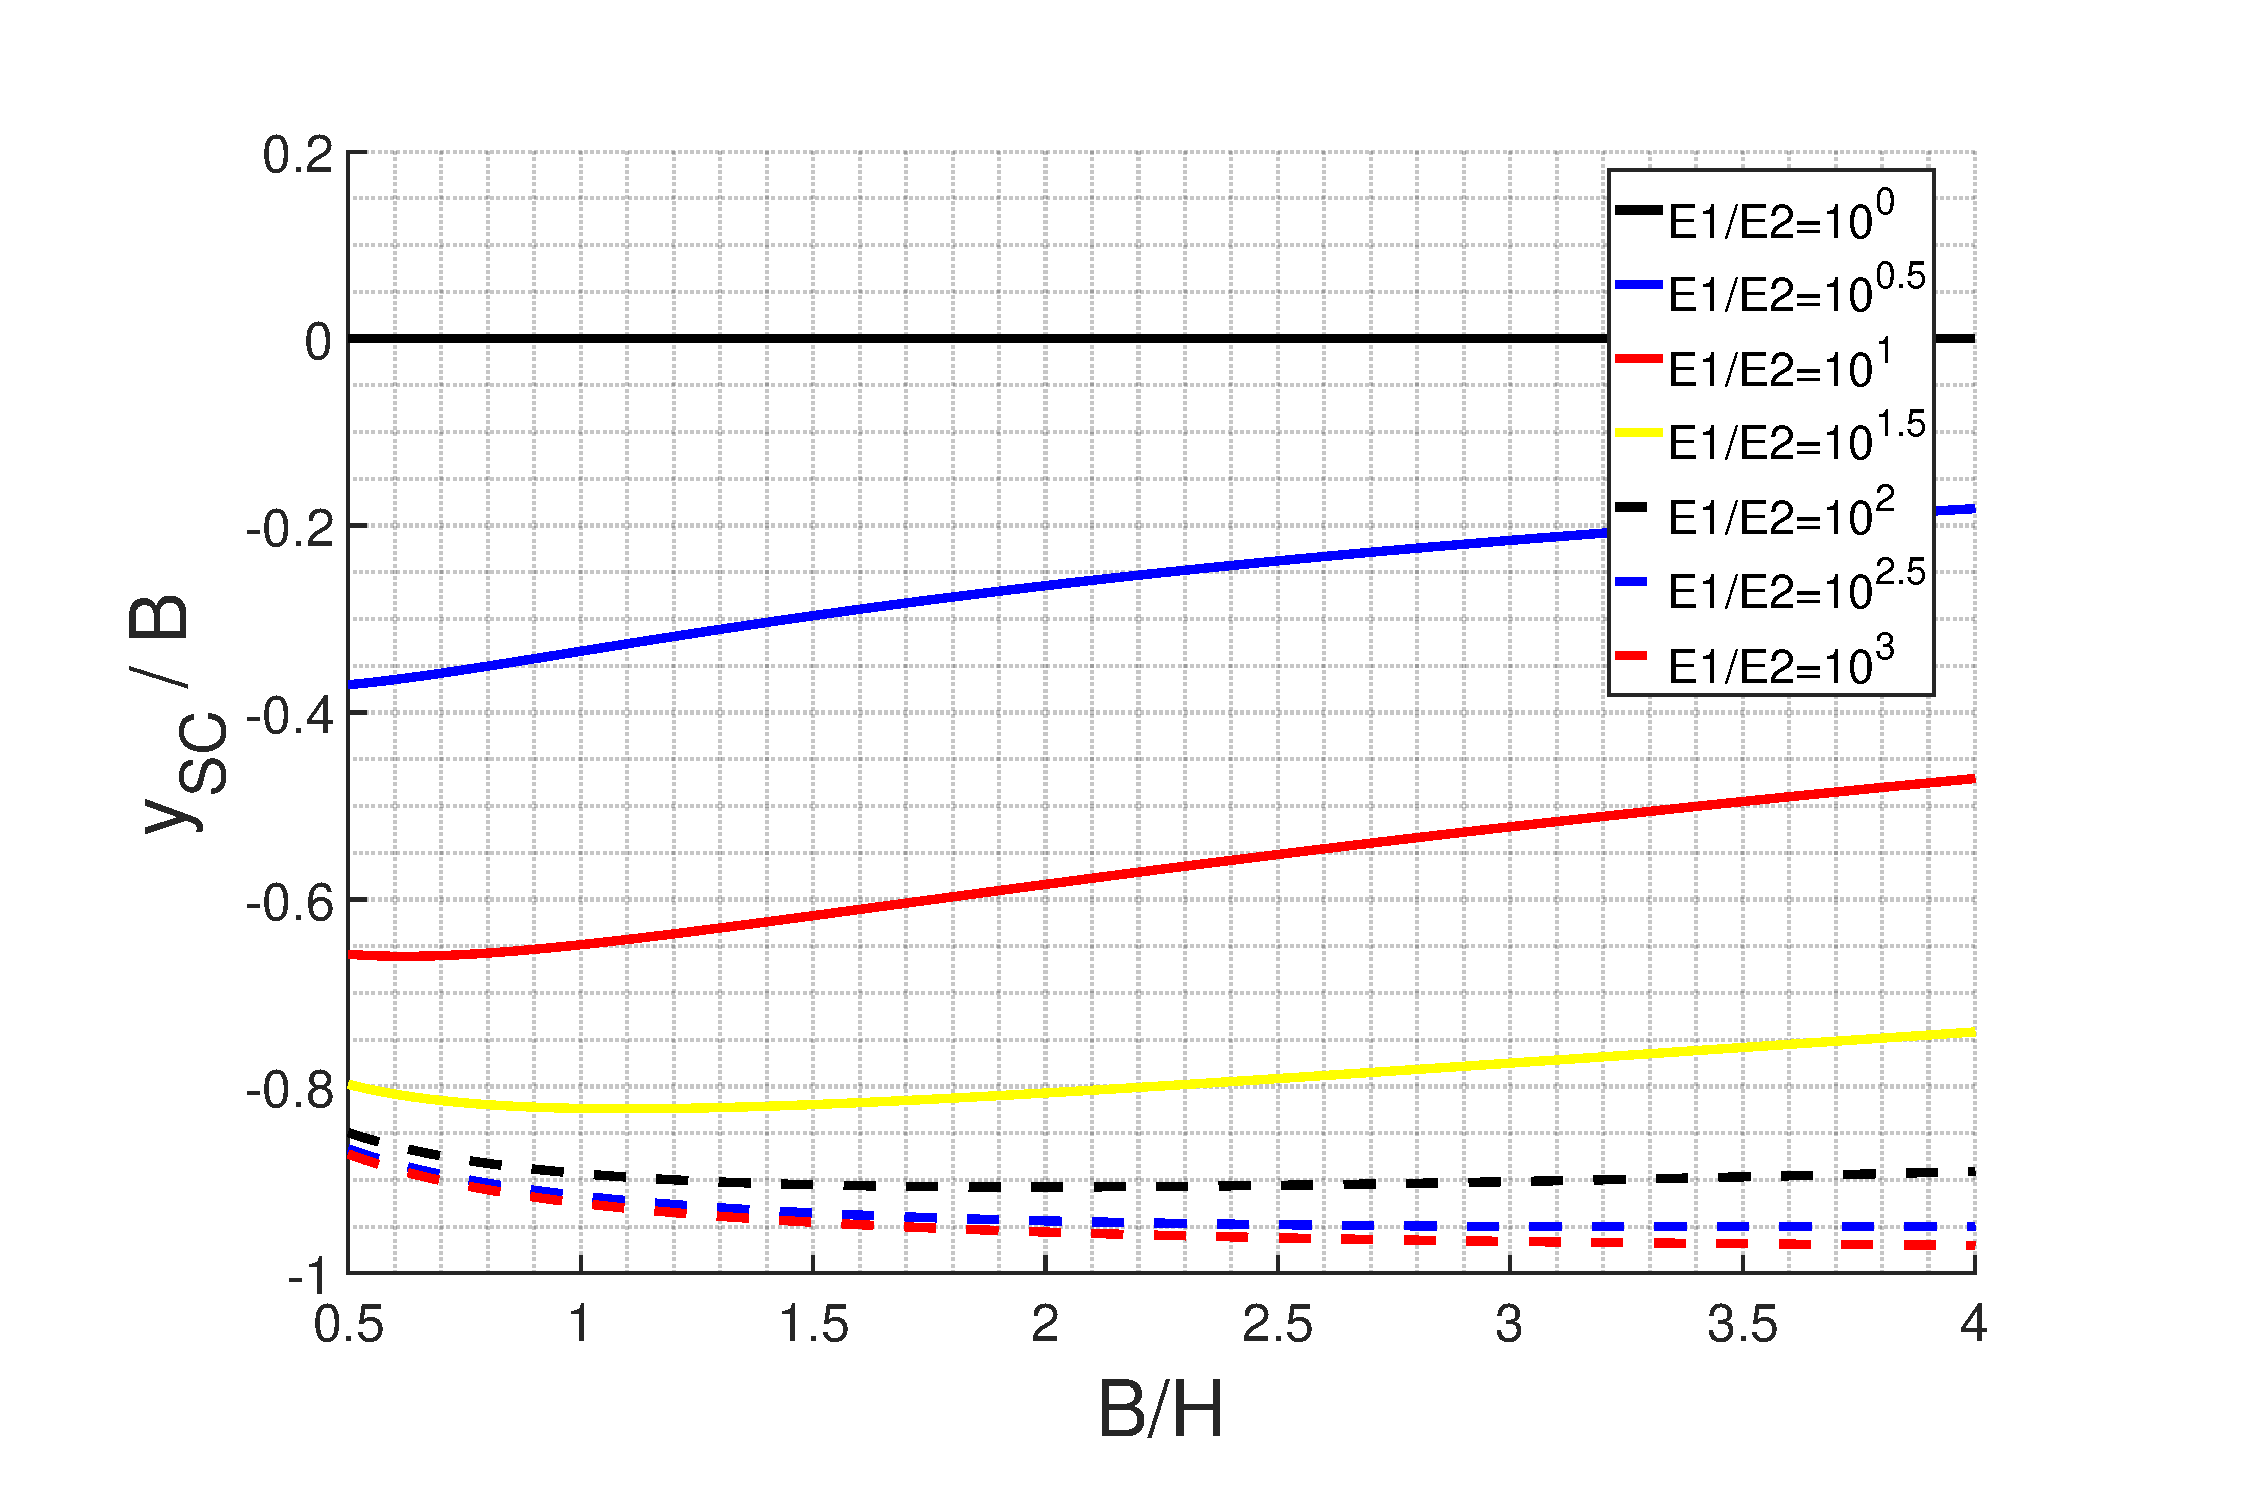
\includegraphics[width=0.8 \textwidth]{../../analytical/figures/SC-E1overE2-BoverH}
  \caption[Influence of the cross-sectional aspect ratio $B/H$ on the dimensionless shear centre position $y_{\mathrm{SC}}/B$]{Influence of the cross-sectional aspect ratio $B/H$ on the dimensionless shear centre position $y_{\mathrm{SC}}/B$ is shown for various values of the stiffness ratio $E_1/E_2$ ranging from $10^0$ to $10^3$. }\label{fig:SC-E1overE2-BoverH}
\end{figure}

\begin{figure}[!htpb] %E I_y = \Phi_y versus B/H
  \centering
  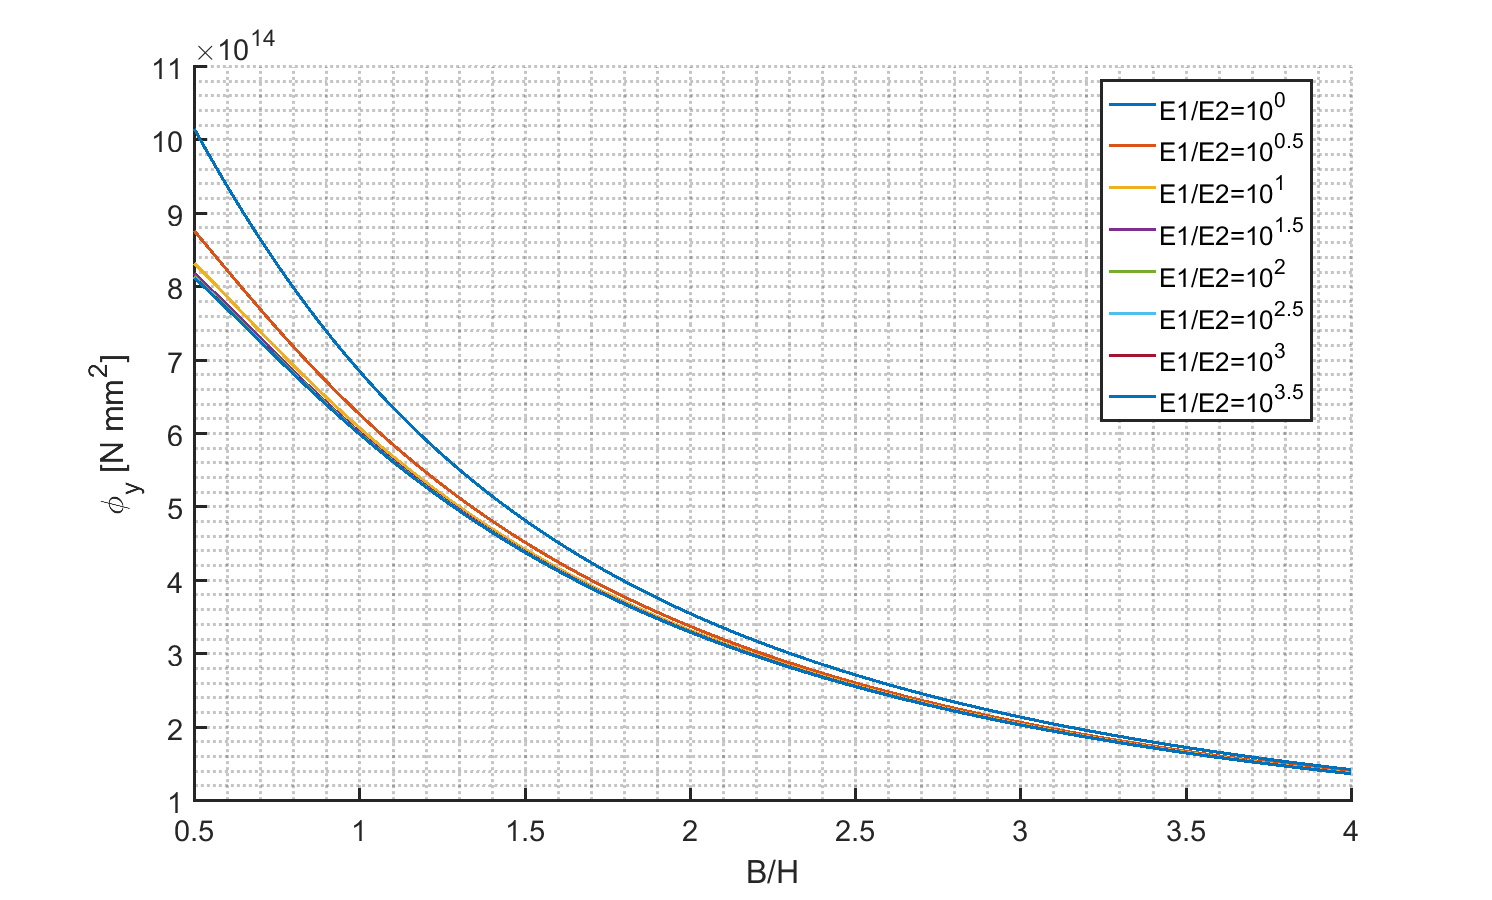
\includegraphics[width=0.8 \textwidth]{../../analytical/figures/EIy-E1overE2-BoverH}
  \caption[Influence of the cross-sectional aspect ratio $B/H$ on the flexural stiffness $EI_y$]{Influence of the cross-sectional aspect ratio $B/H$ on the flexural stiffness $EI_y = \Phi_y$ is shown for various values of the stiffness ratio $E_1/E_2$ ranging from $10^0$ to $10^3$. }\label{fig:EIy-E1overE2-BoverH}
\end{figure}

\begin{figure}[!htpb] %w_0,tip / Q versus B/H, deflection compliance
  \centering
  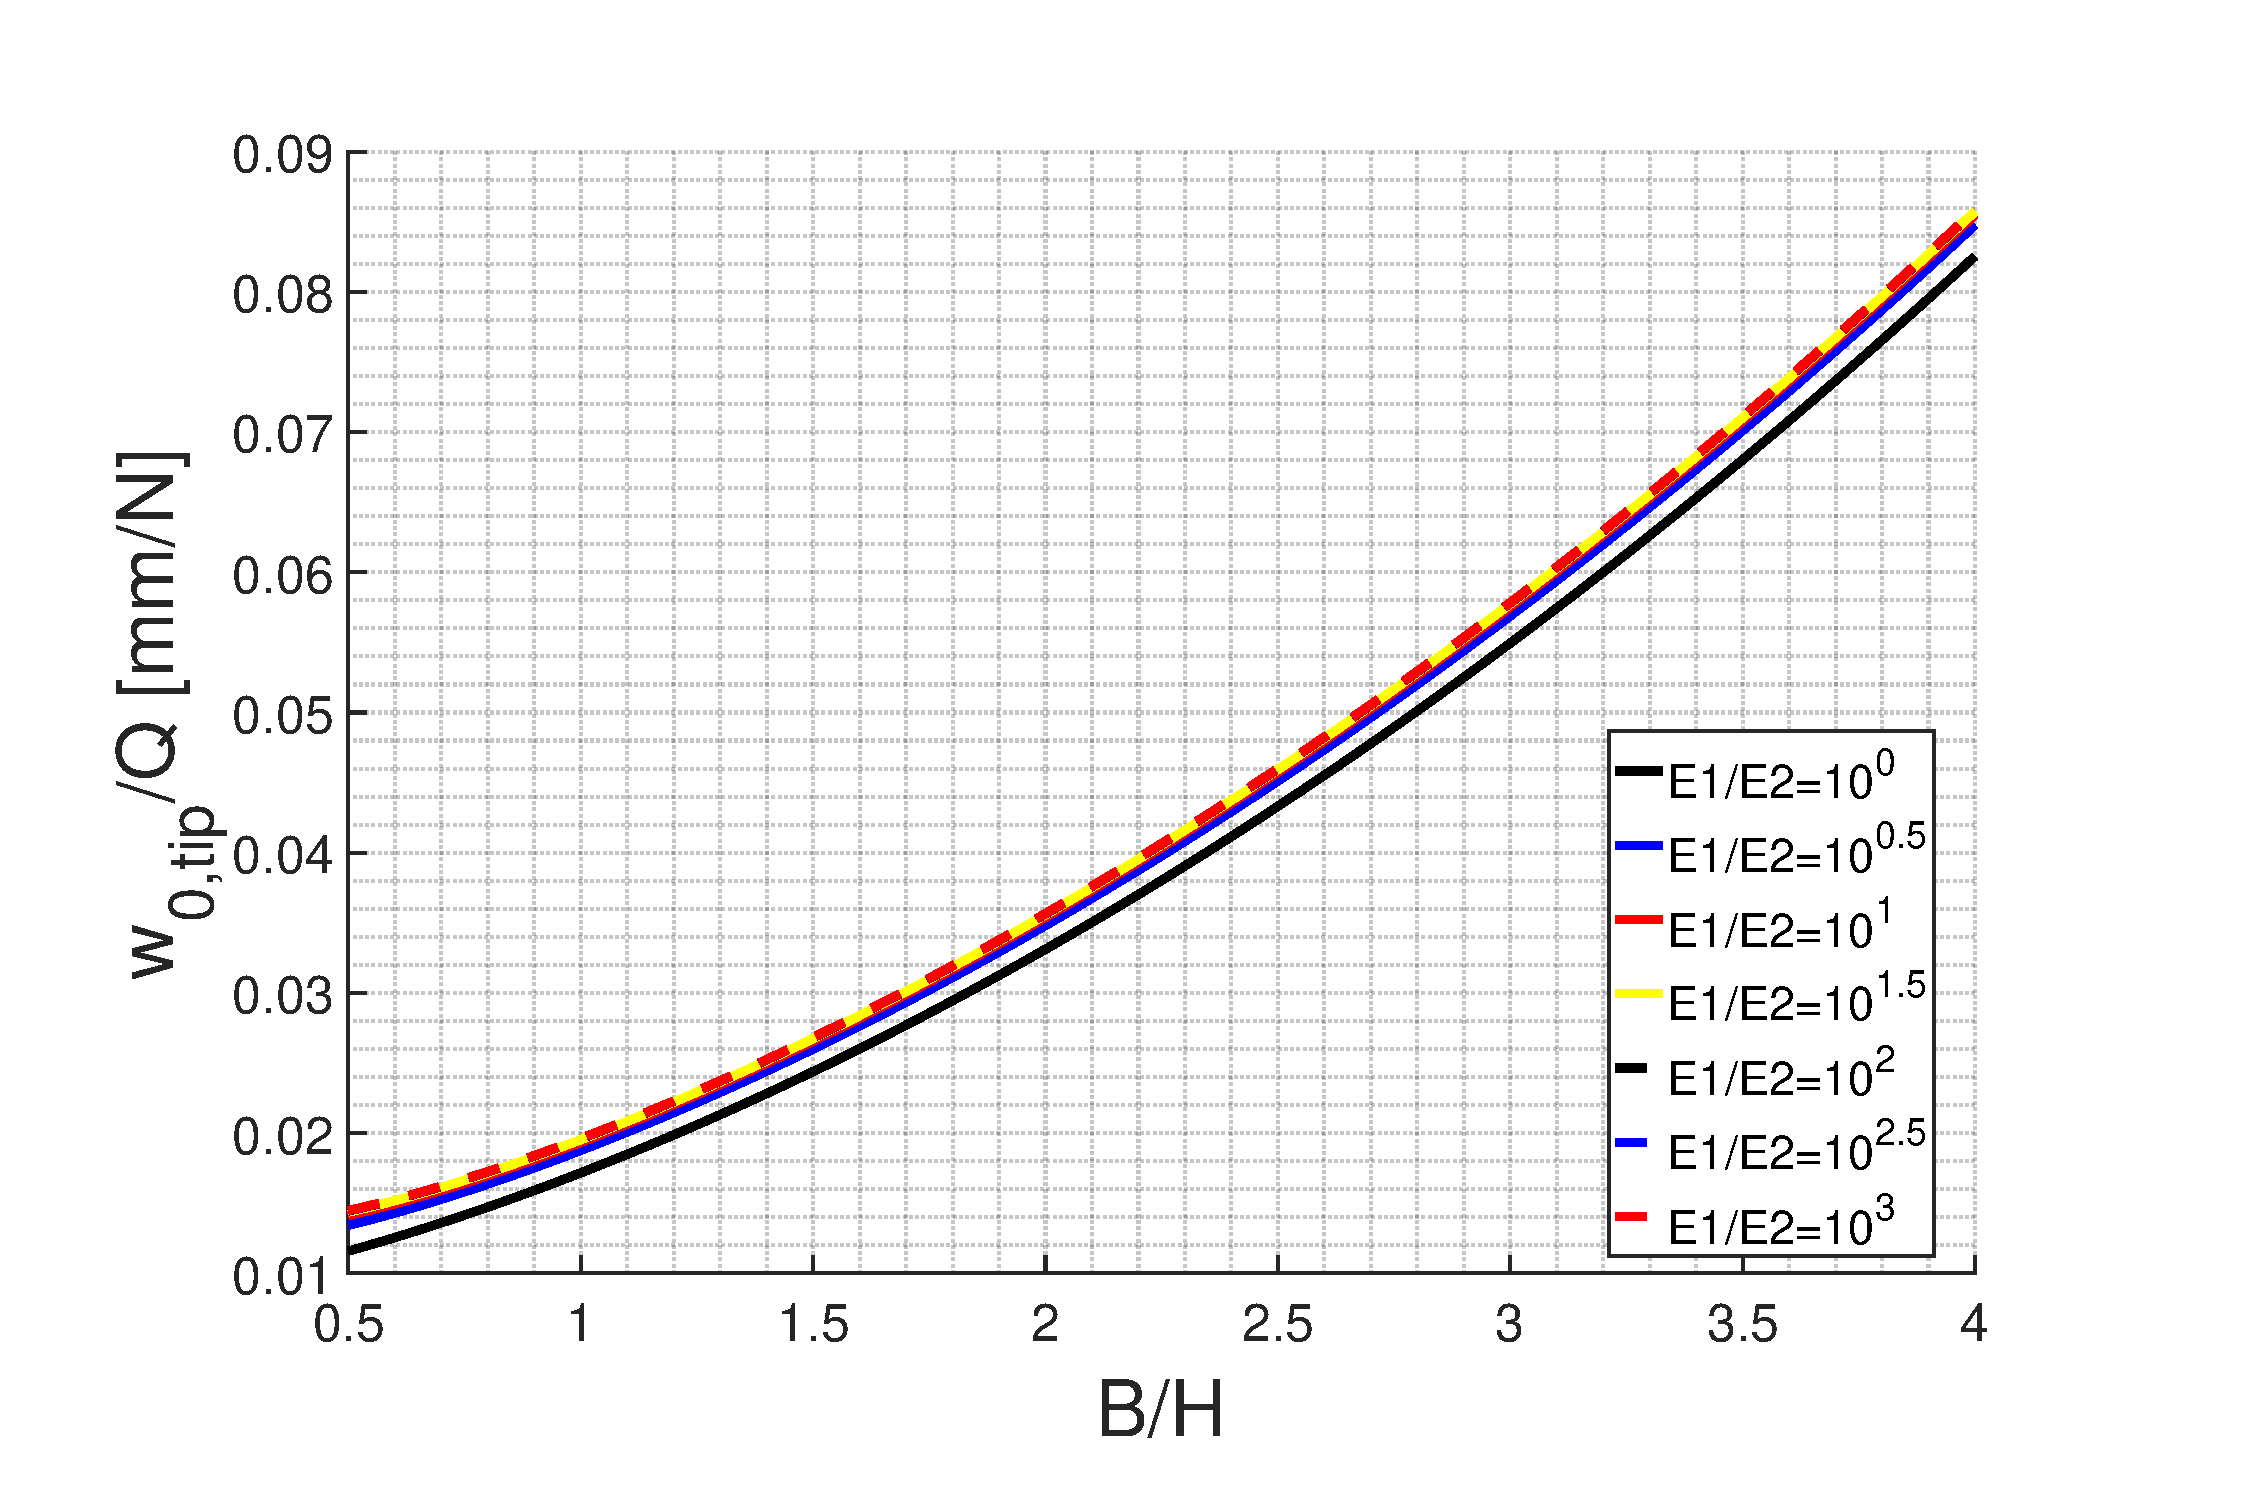
\includegraphics[width=0.8 \textwidth]{../../analytical/figures/woverQ-E1overE2-BoverH}
  \caption[Influence of the cross-sectional aspect ratio $B/H$ on the deflection compliance]{Influence of the cross-sectional aspect ratio $B/H$ on the deflection compliance $w_{\mathrm{0,tip}} / Q$ is shown for various values of the stiffness ratio $E_1/E_2$ ranging from $10^0$ to $10^3$. }\label{fig:woverQ-E1overE2-BoverH}
\end{figure}

\begin{figure}[!htpb] %\phi_tip / Q versus B/H, torsional compliance
  \centering
  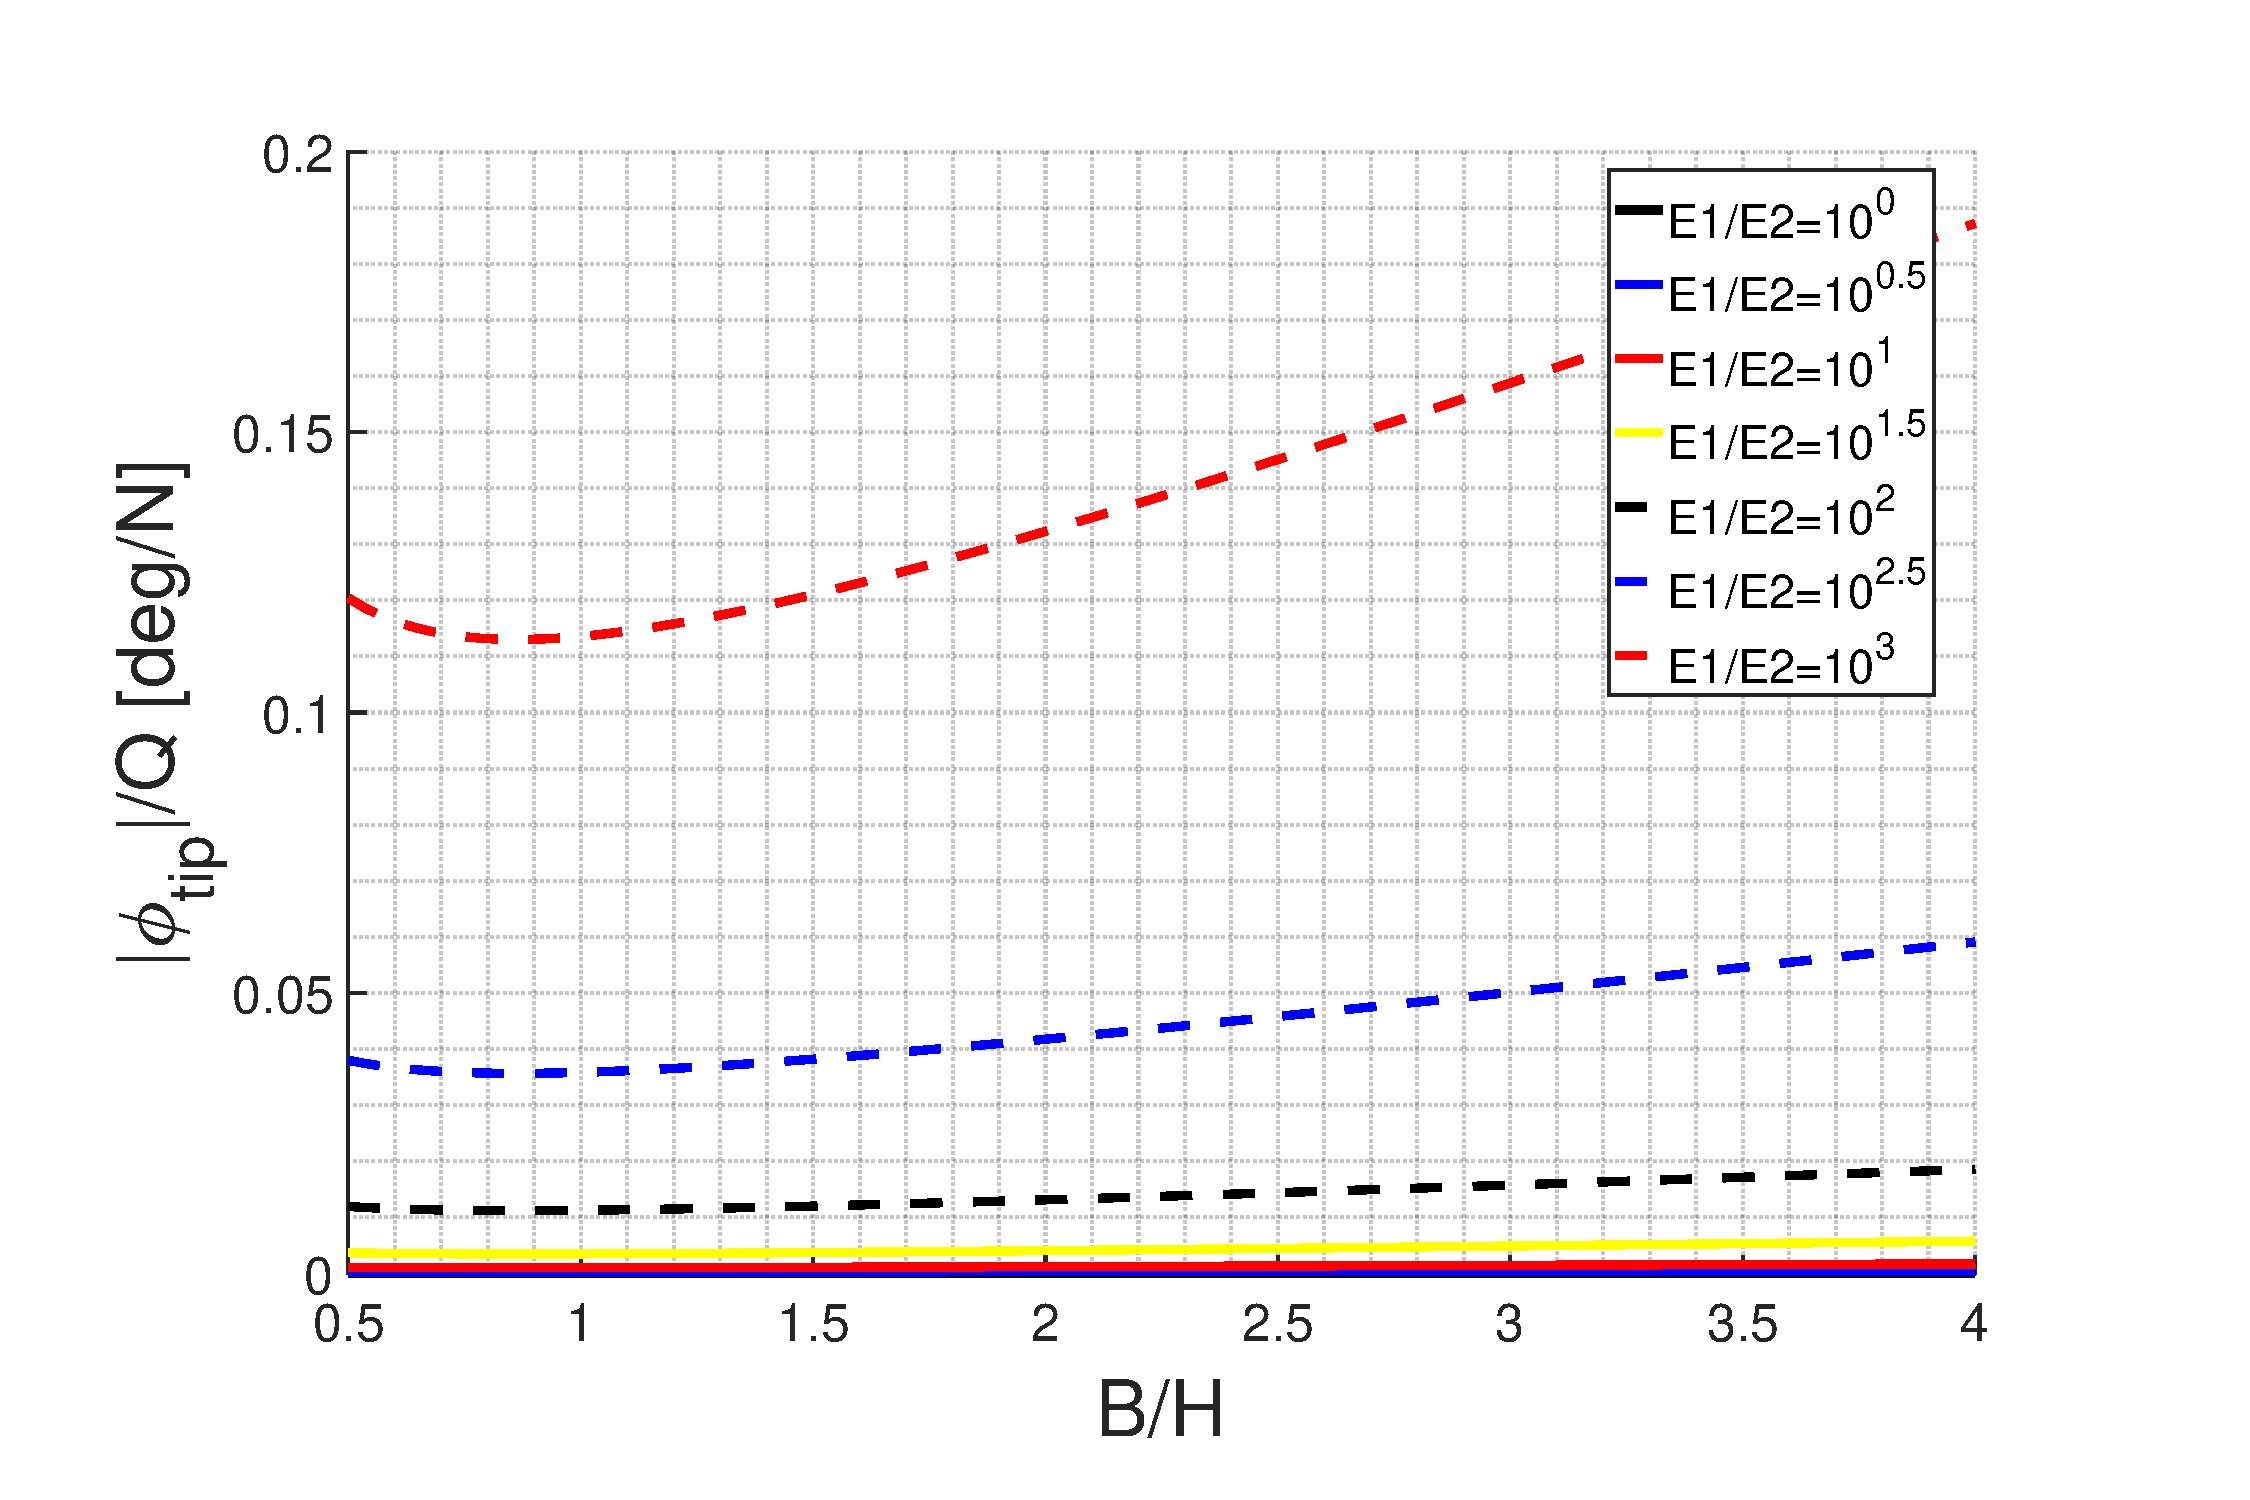
\includegraphics[width=0.8 \textwidth]{../../analytical/figures/phioverQ-E1overE2-BoverH}
  \caption[Influence of the cross-sectional aspect ratio $B/H$ on the torsional compliance]{Influence of the cross-sectional aspect ratio $B/H$ on the torsional compliance $|\phi_{\mathrm{tip}}| / Q$ is shown for various values of the stiffness ratio $E_1/E_2$ ranging from $10^0$ to $10^3$. }\label{fig:phioverQ-E1overE2-BoverH}
\end{figure}

%%%% Figures variation of t2/t1
\begin{figure}[!htpb] %G I_t versus t2/t1
  \centering
  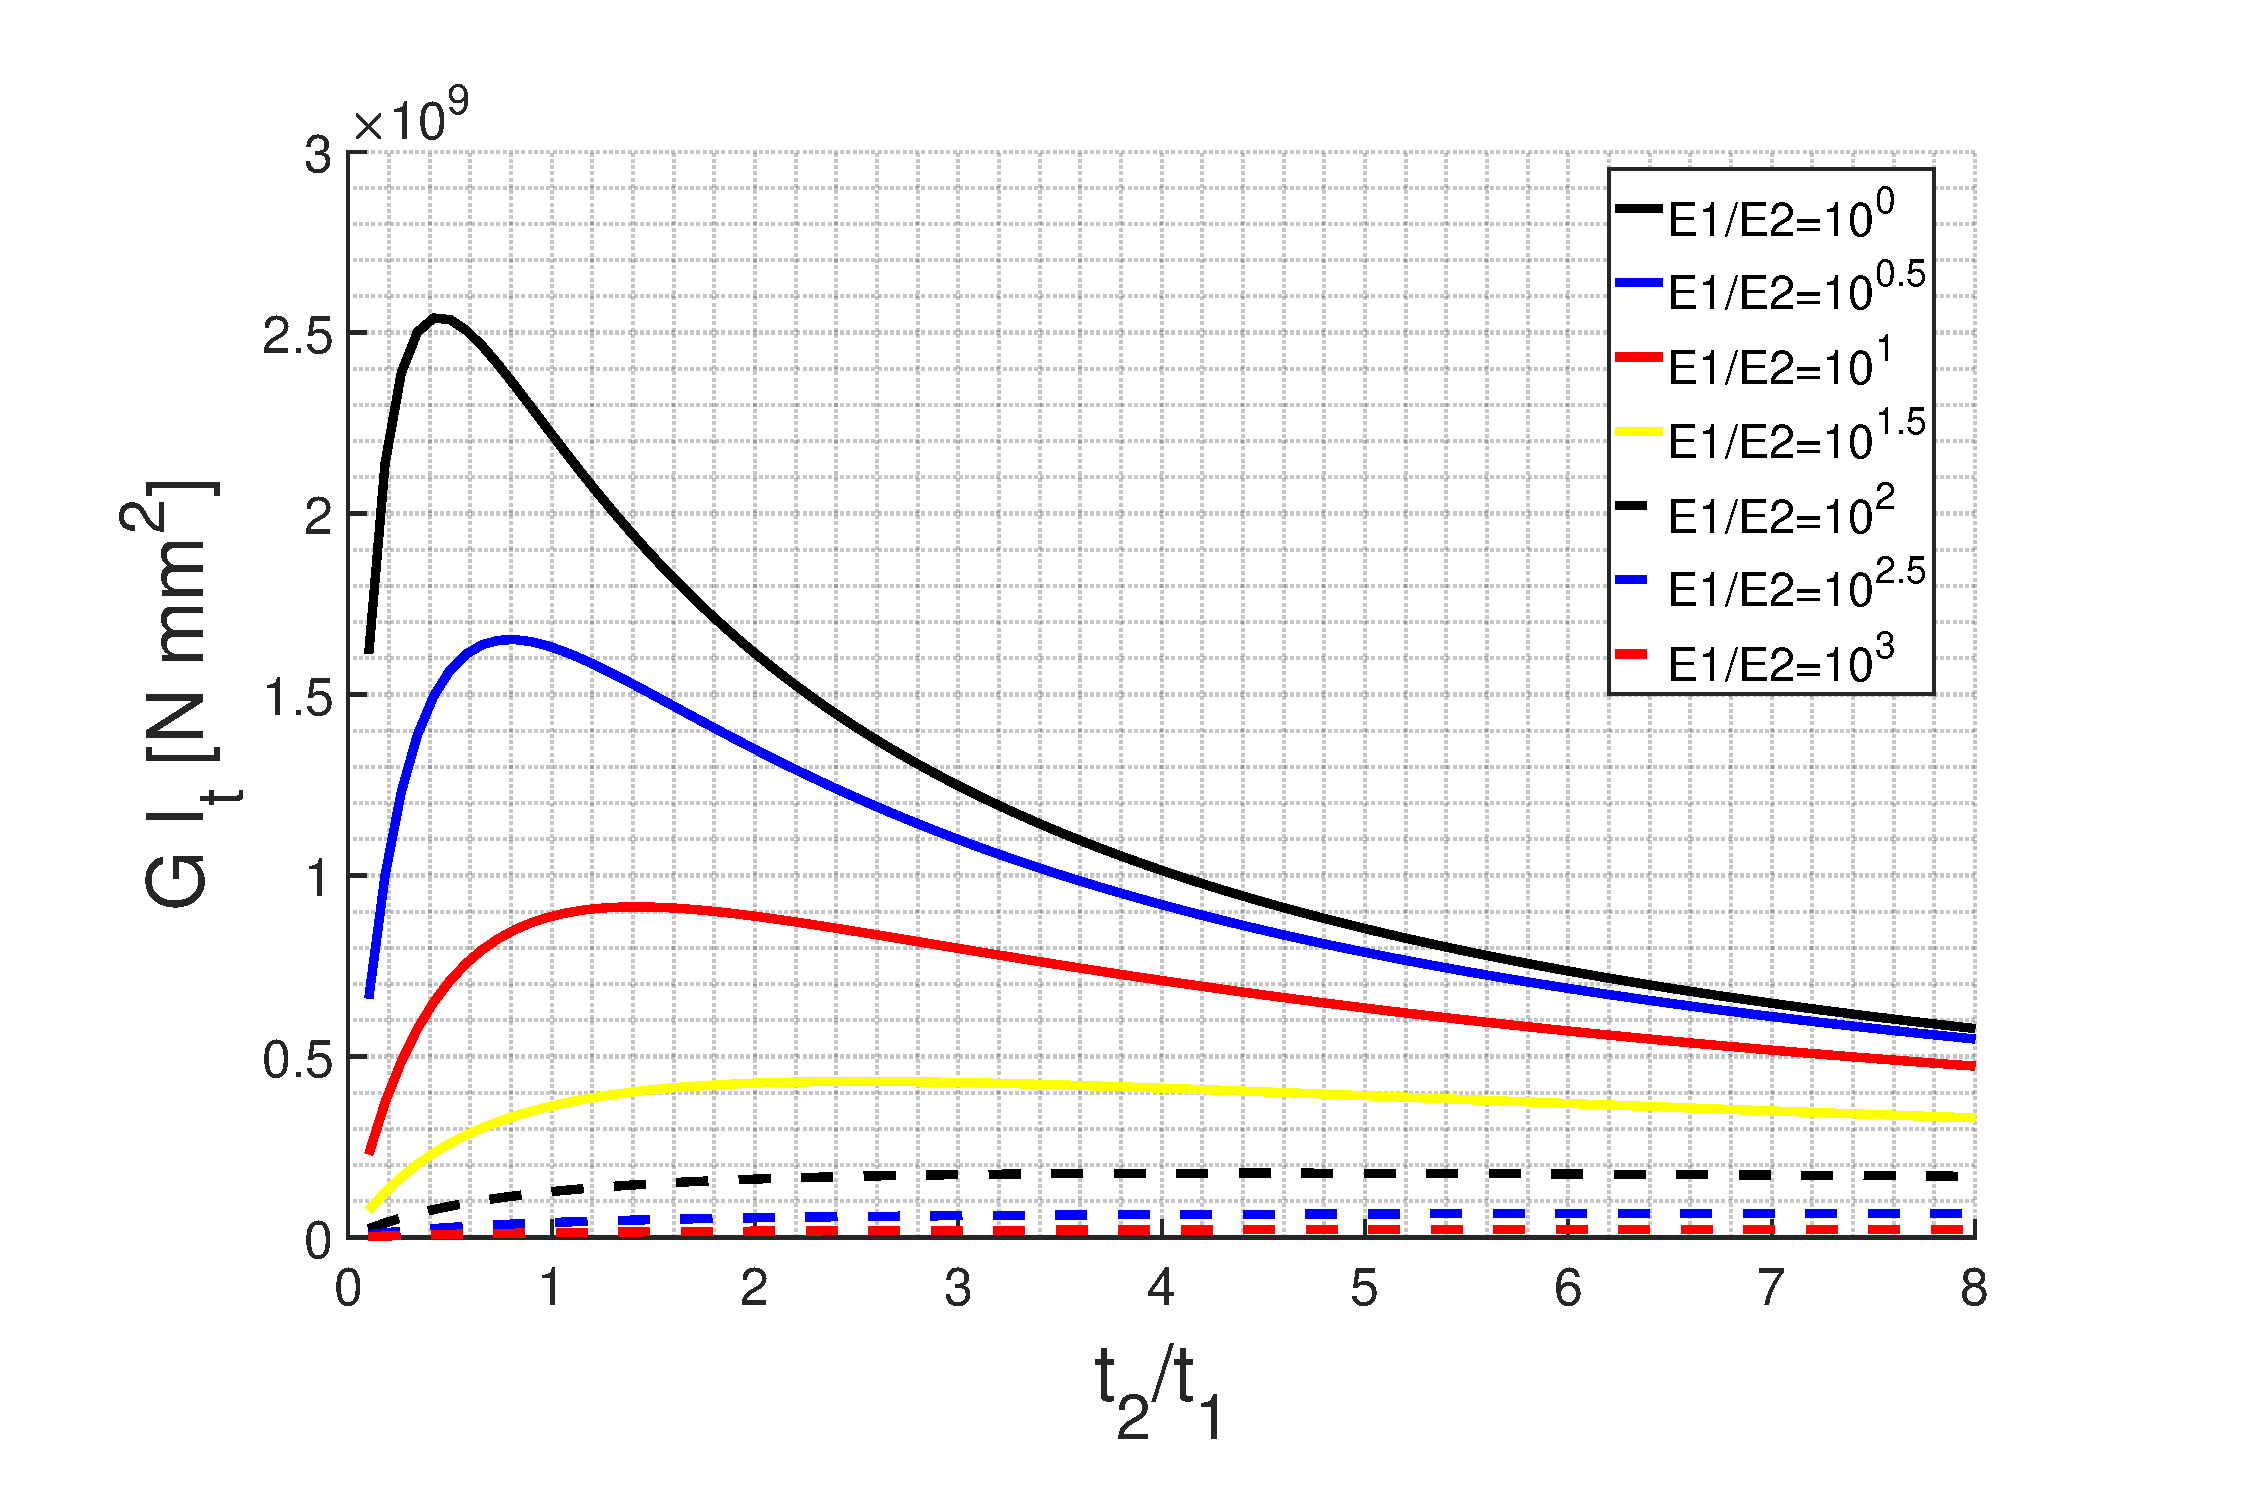
\includegraphics[width=0.8 \textwidth]{../../analytical/figures/GIt-E1overE2-t2overt1}
  \caption[Influence of the wall thickness ratio $t_2/t_1$ on the torsional stiffness $GI_t$]{Influence of the wall thickness ratio $t_2/t_1$ on the torsional stiffness $GI_t$ shown for various values of the stiffness ratio $E_1/E_2$ ranging from $10^0$ to $10^3$. }\label{fig:GIt-E1overE2-t2overt1}
\end{figure}

\begin{figure}[!htpb] %Shear centre versus t2/t1
  \centering
  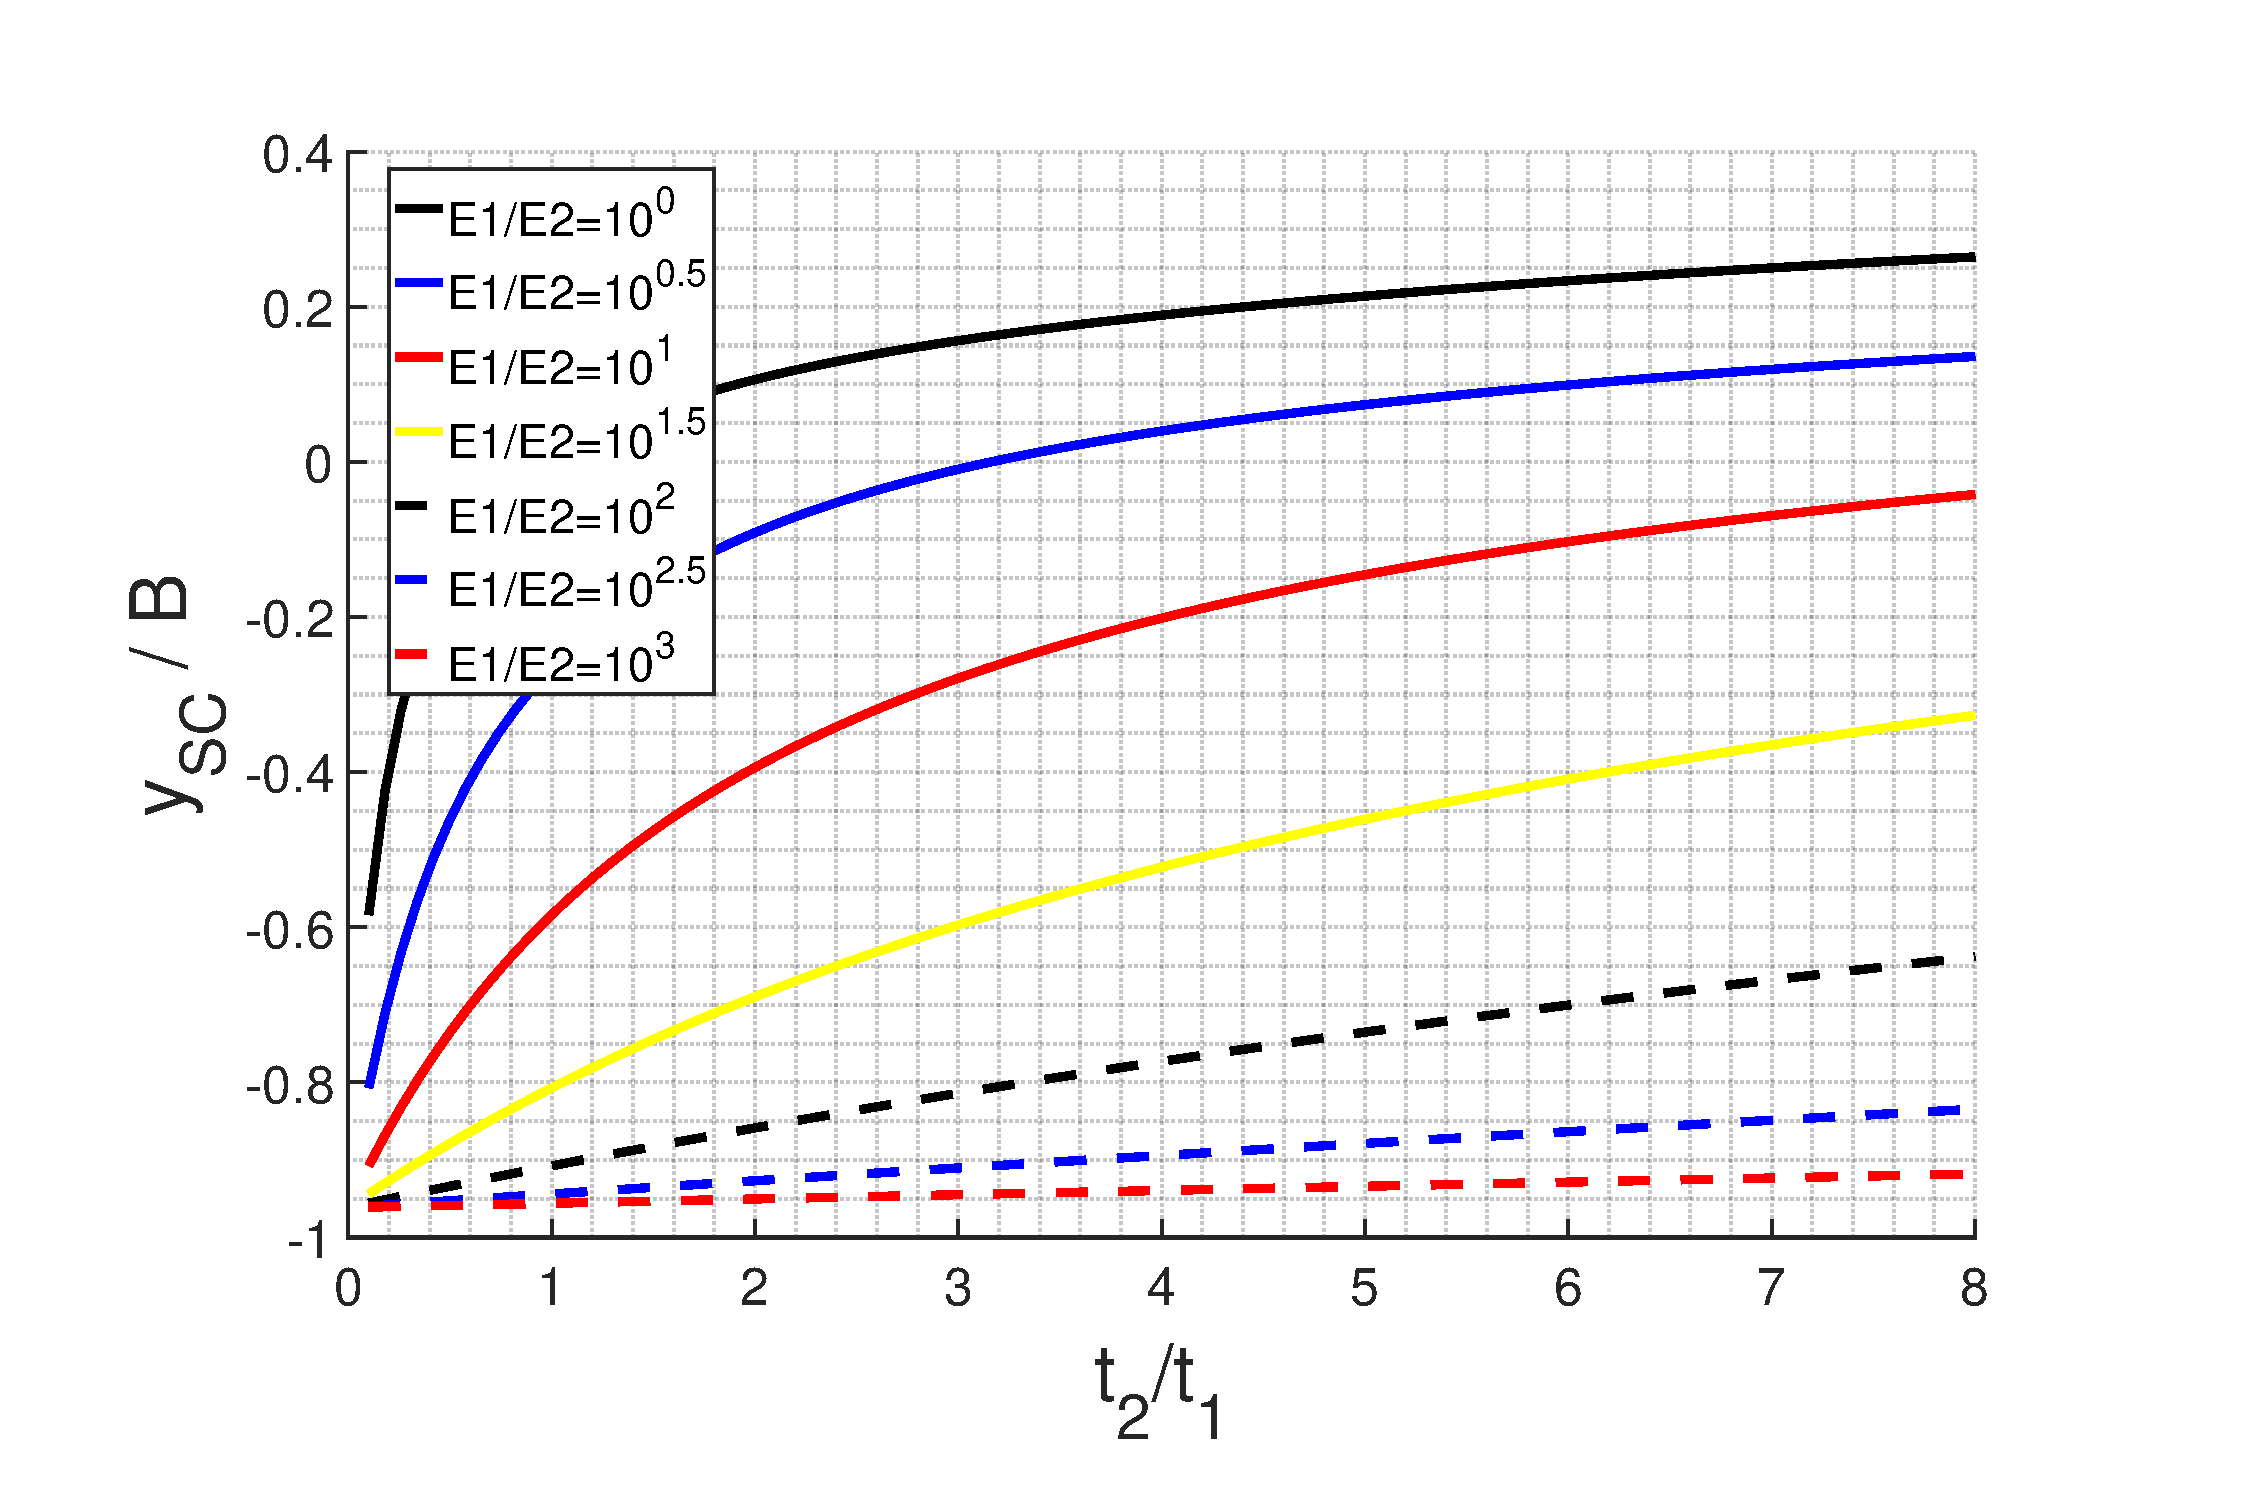
\includegraphics[width=0.8 \textwidth]{../../analytical/figures/SC-E1overE2-t2overt1}
  \caption[Influence of the wall thickness ratio $t_2/t_1$ on the dimensionless shear centre position $y_{\mathrm{SC}}/B$]{Influence of the wall thickness ratio $t_2/t_1$ on the dimensionless shear centre position $y_{\mathrm{SC}}/B$ shown for various values of the stiffness ratio $E_1/E_2$ ranging from $10^0$ to $10^3$. }\label{fig:SC-E1overE2-t2overt1}
\end{figure}

\begin{figure}[!htpb] %E I_y = \Phi_y versus t2/t1
  \centering
  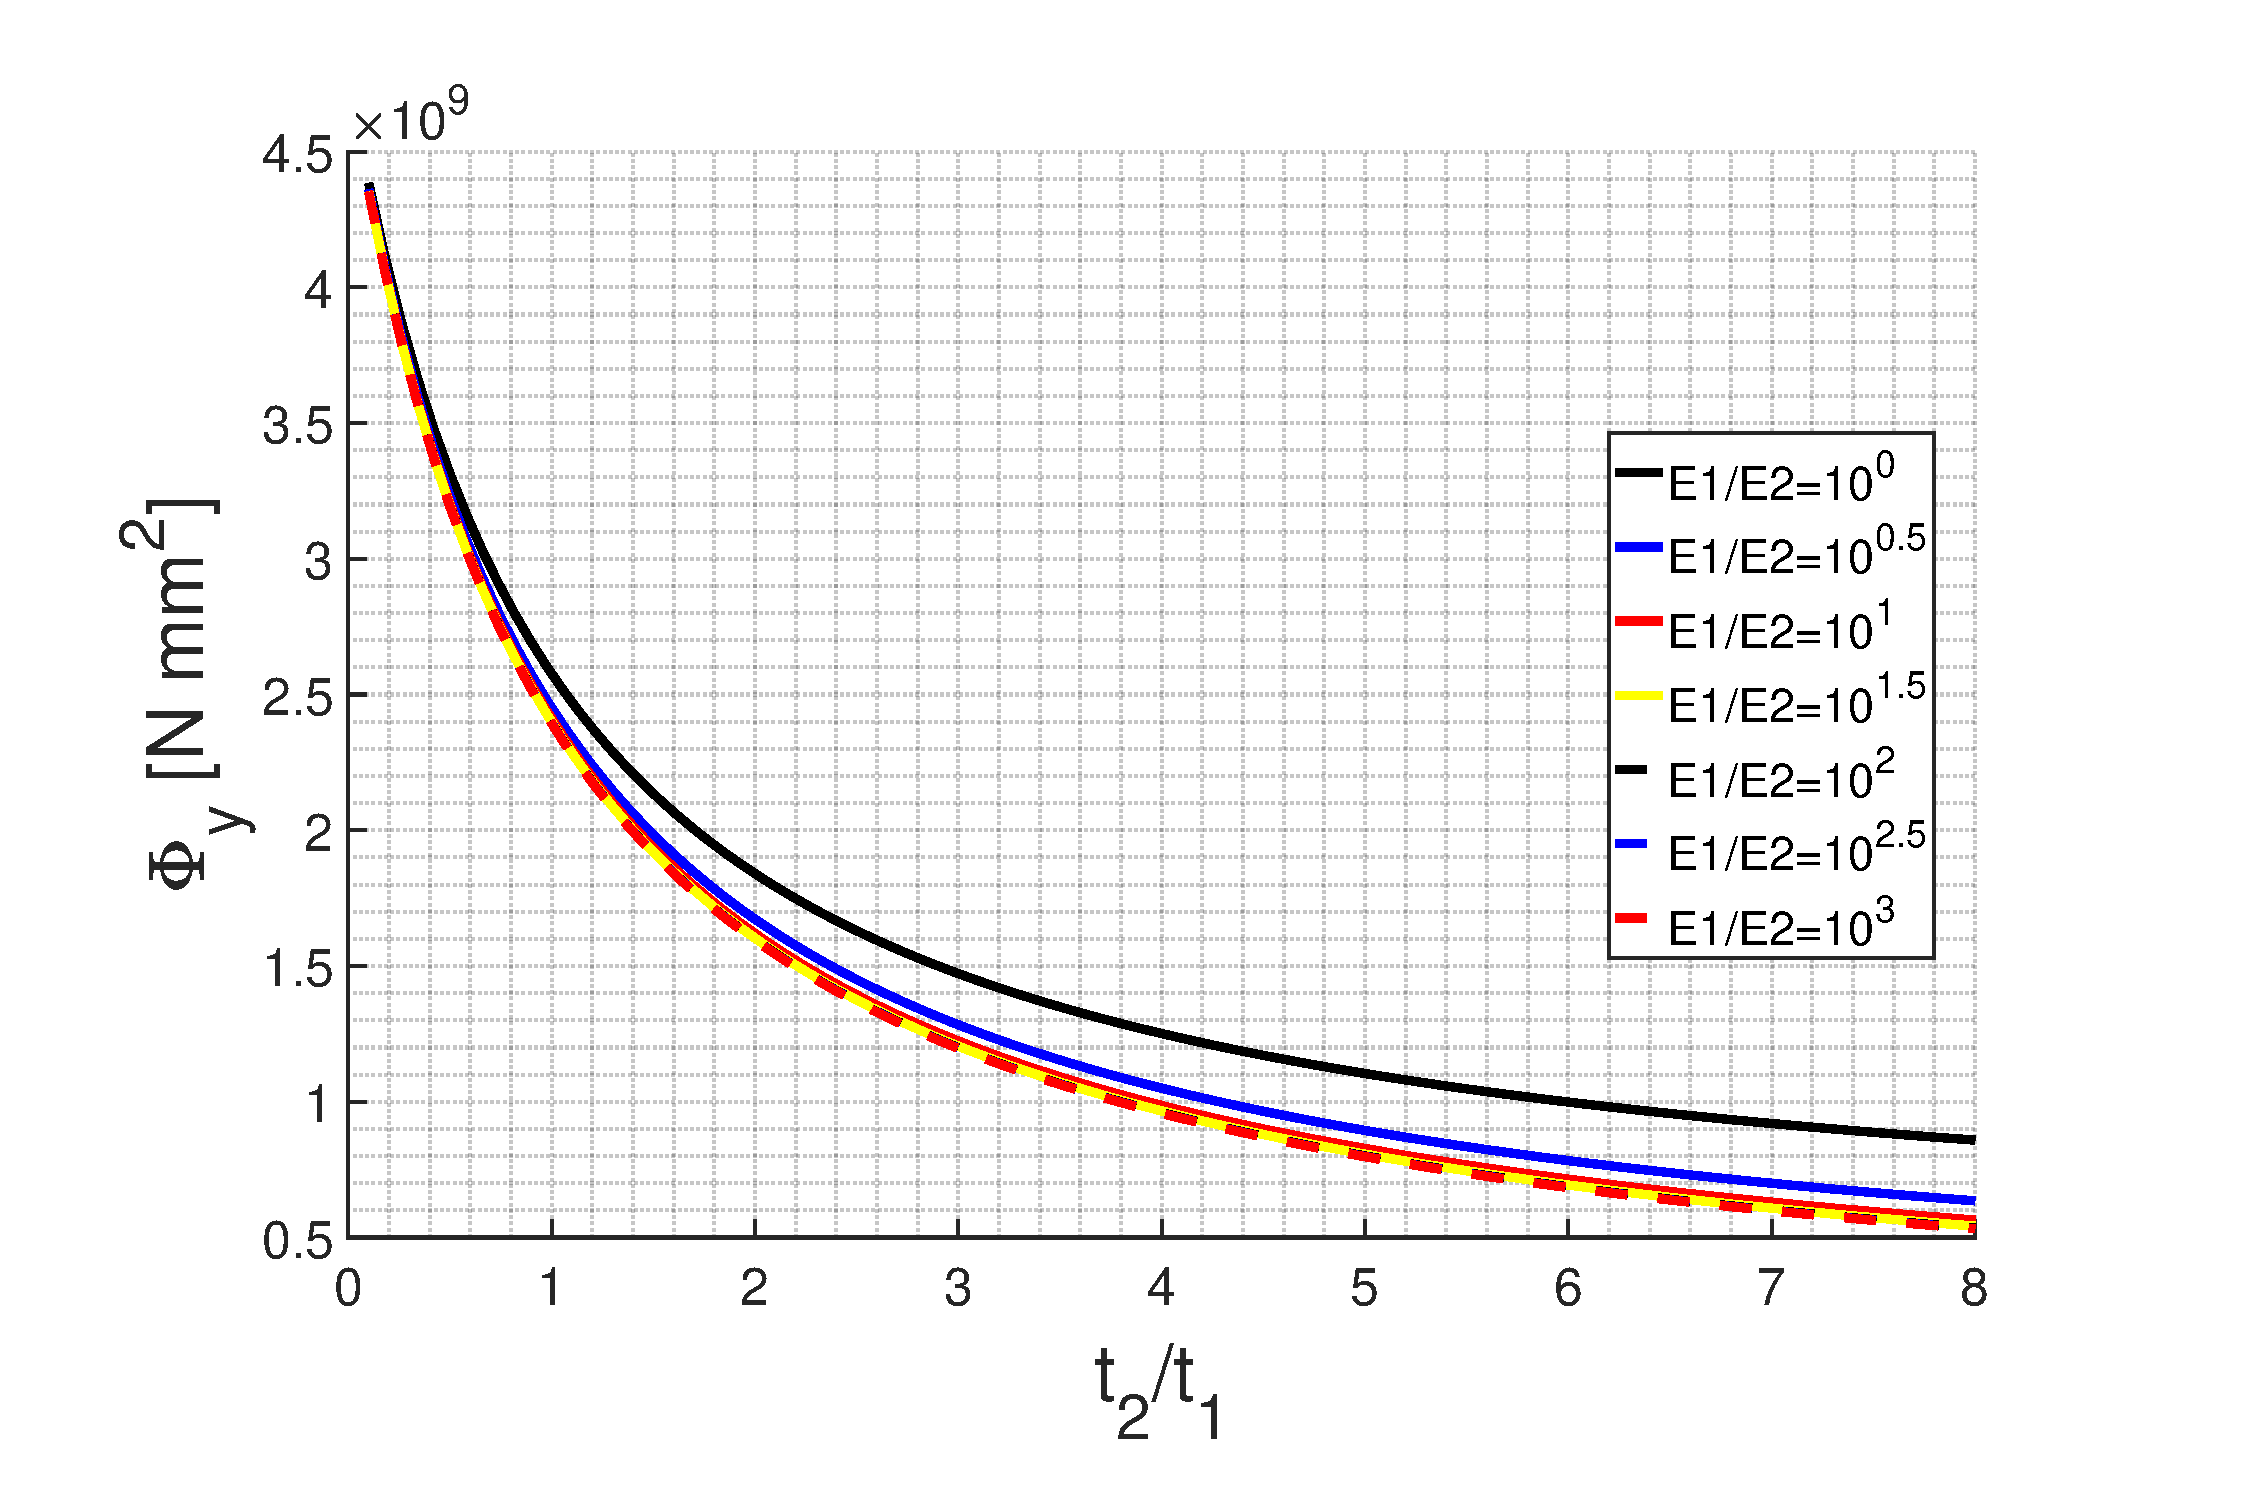
\includegraphics[width=0.8 \textwidth]{../../analytical/figures/EIy-E1overE2-t2overt1}
  \caption[Influence of the wall thickness ratio $t_2/t_1$ on the flexural stiffness $EI_y$]{Influence of the wall thickness ratio $t_2/t_1$ on the flexural stiffness $EI_y = \Phi_y$ shown for various values of the stiffness ratio $E_1/E_2$ ranging from $10^0$ to $10^3$. }\label{fig:EIy-E1overE2-t2overt1}
\end{figure}

\begin{figure}[!htpb] %w_0,tip / Q versus t2/t1, deflection compliance
  \centering
  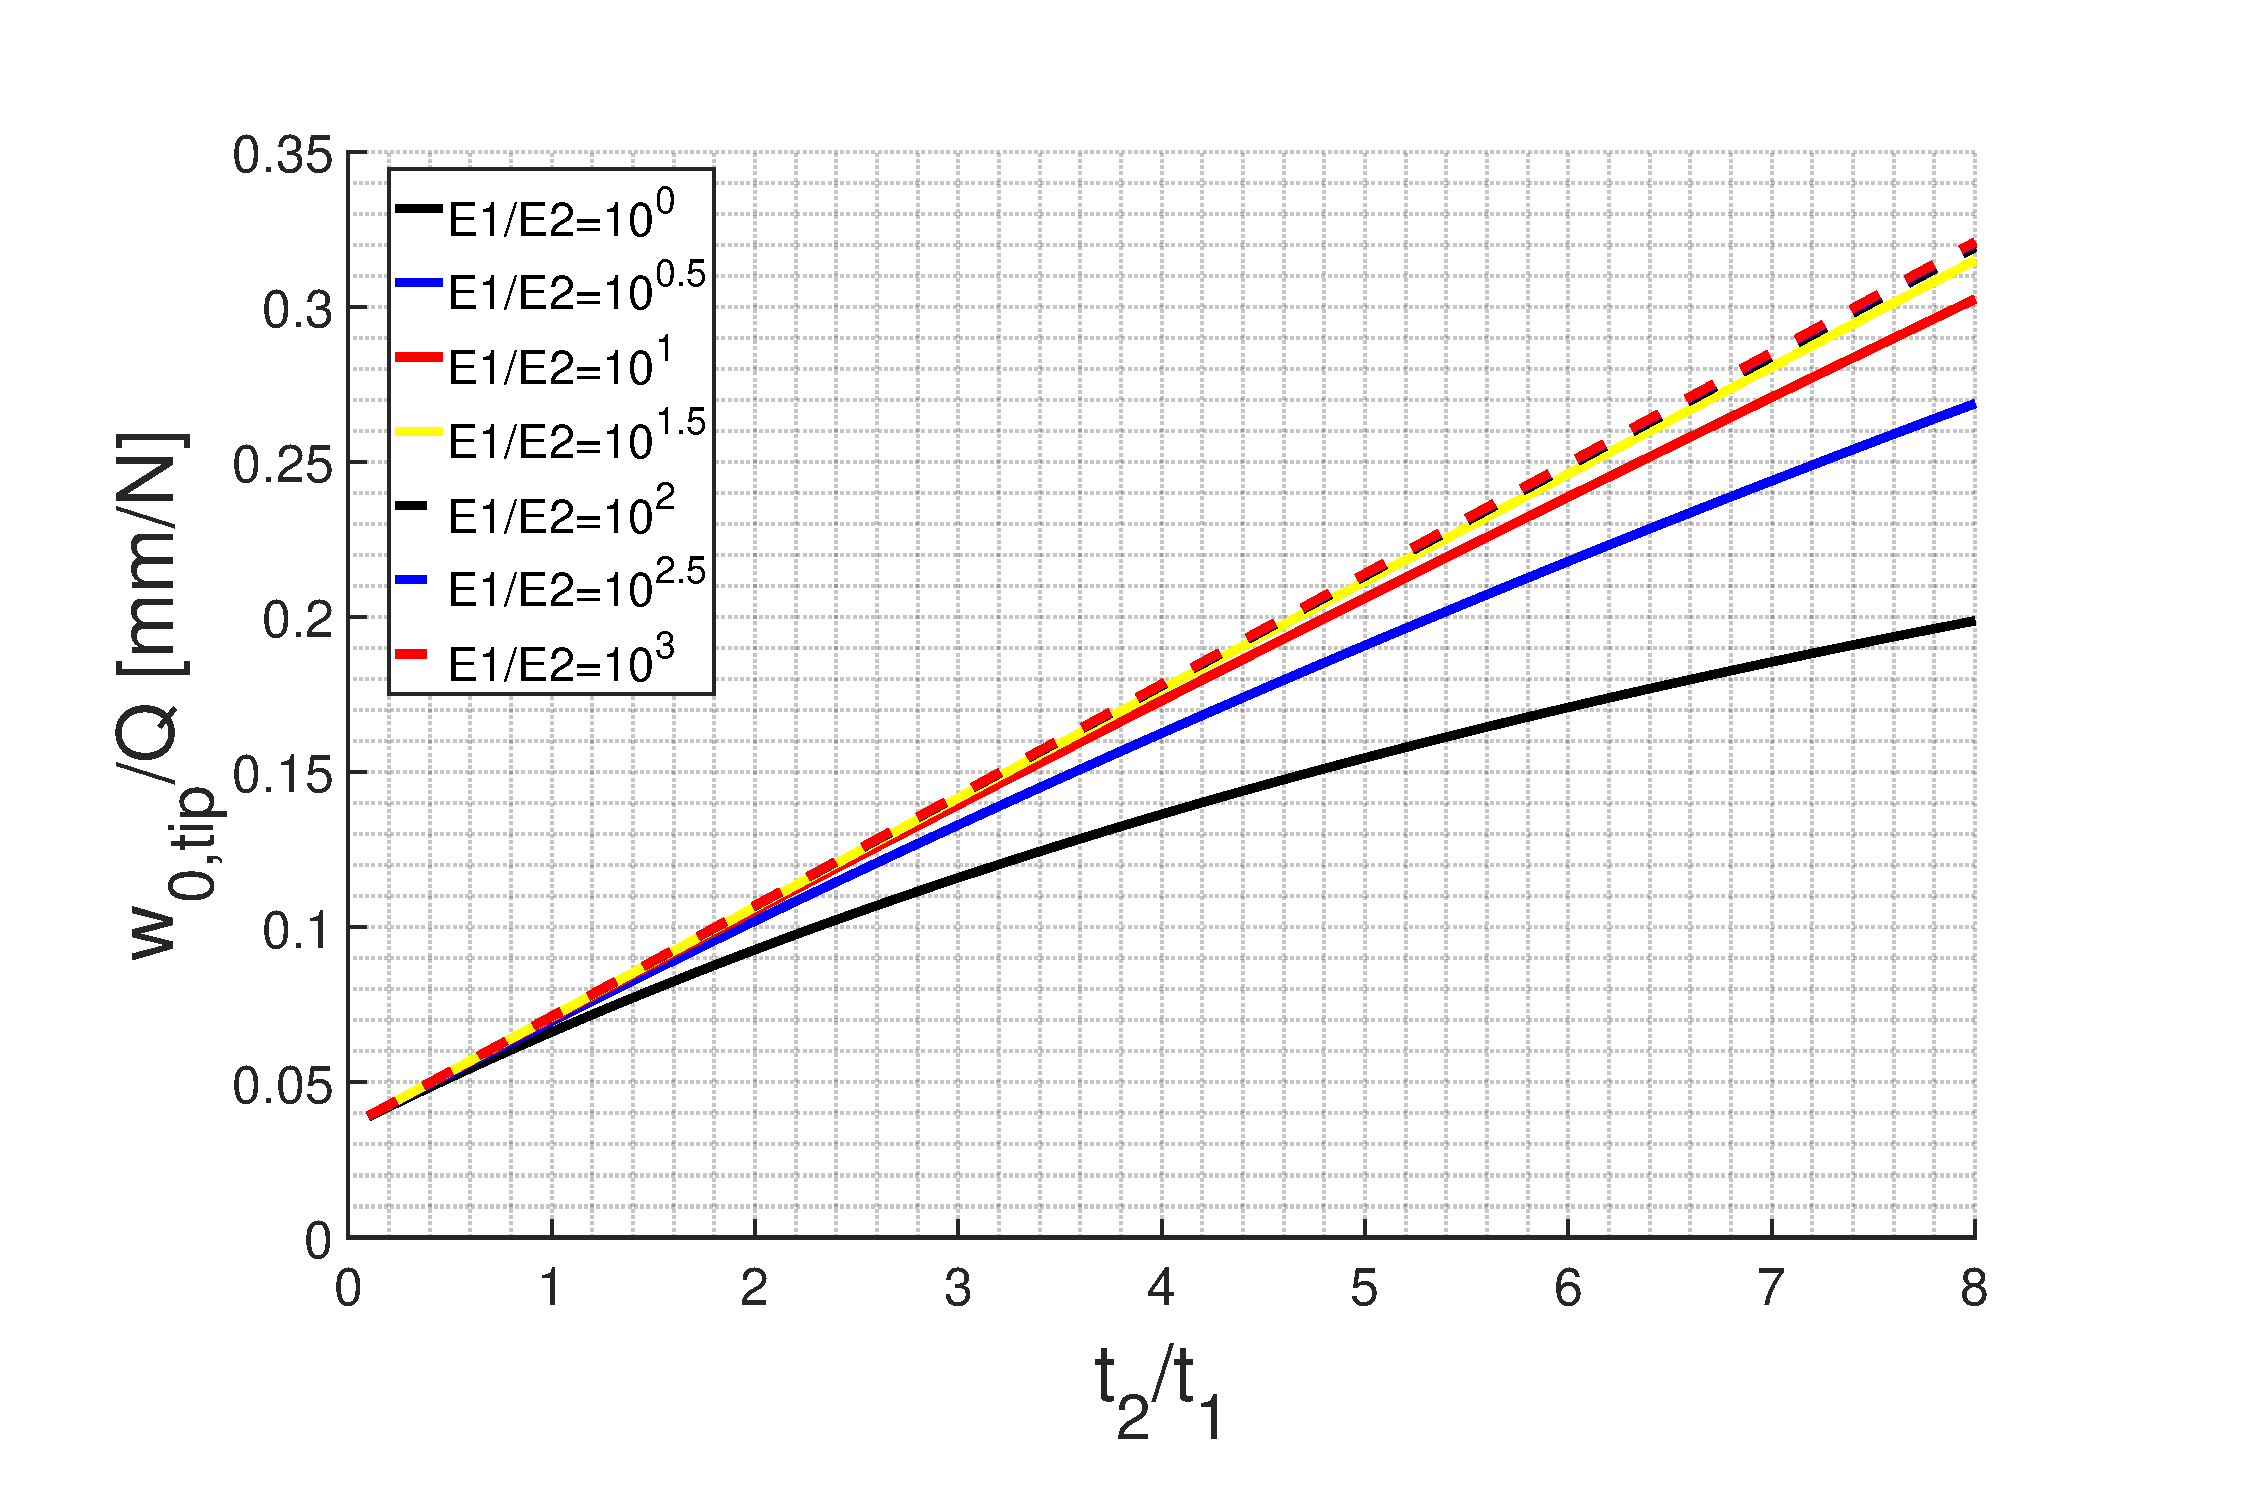
\includegraphics[width=0.8 \textwidth]{../../analytical/figures/woverQ-E1overE2-t2overt1}
  \caption[Influence of the thickness ratio $t2/t1$ on the deflection compliance]{Influence of the thickness ratio $t2/t1$ on the deflection compliance $w_{\mathrm{0,tip}} / Q$ is shown for various values of the stiffness ratio $E_1/E_2$ ranging from $10^0$ to $10^3$. }\label{fig:woverQ-E1overE2-t2overt1}
\end{figure}

\begin{figure}[!htpb] %\phi_tip / Q versus t2/t1, torsional compliance
  \centering
  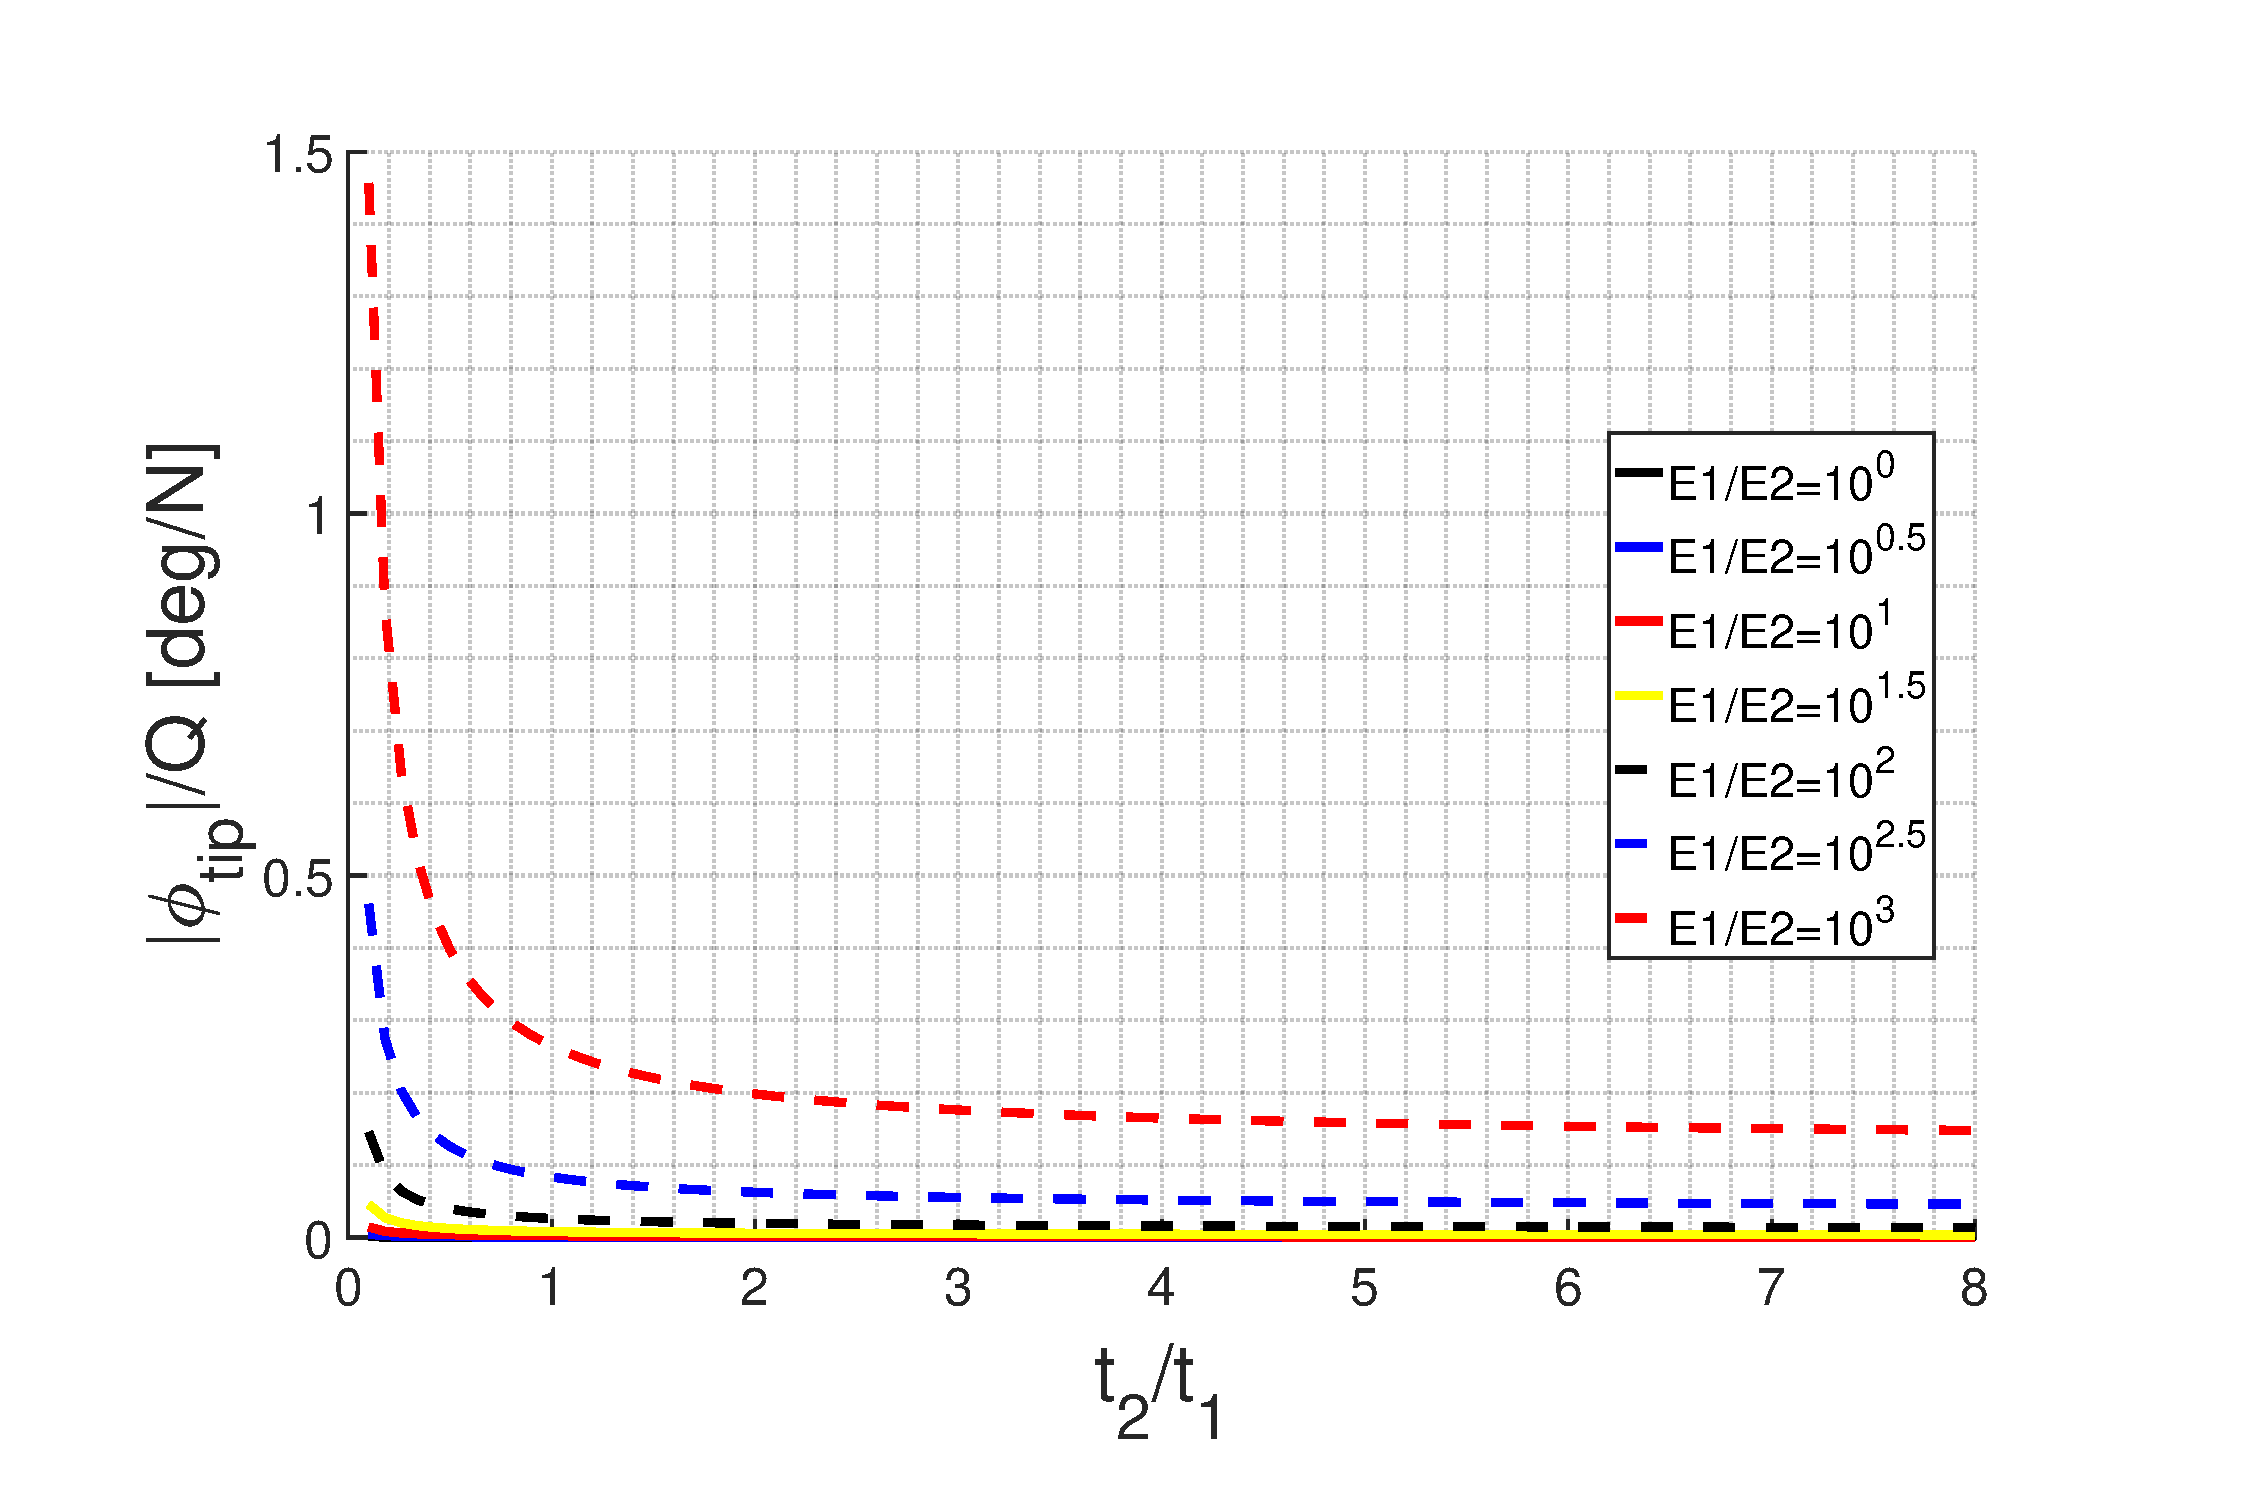
\includegraphics[width=0.8 \textwidth]{../../analytical/figures/phioverQ-E1overE2-t2overt1}
  \caption[Influence of the thickness ratio $t2/t1$ on the torsional compliance]{Influence of the thickness ratio $t2/t1$ on the torsional compliance $|\phi_{\mathrm{tip}}| / Q$ is shown for various values of the stiffness ratio $E_1/E_2$ ranging from $10^0$ to $10^3$. }\label{fig:phioverQ-E1overE2-t2overt1}
\end{figure}

%%%% Figures variation of L / B
\begin{figure}[!htpb] %w_0,tip / Q versus L/B, deflection compliance
  \centering
  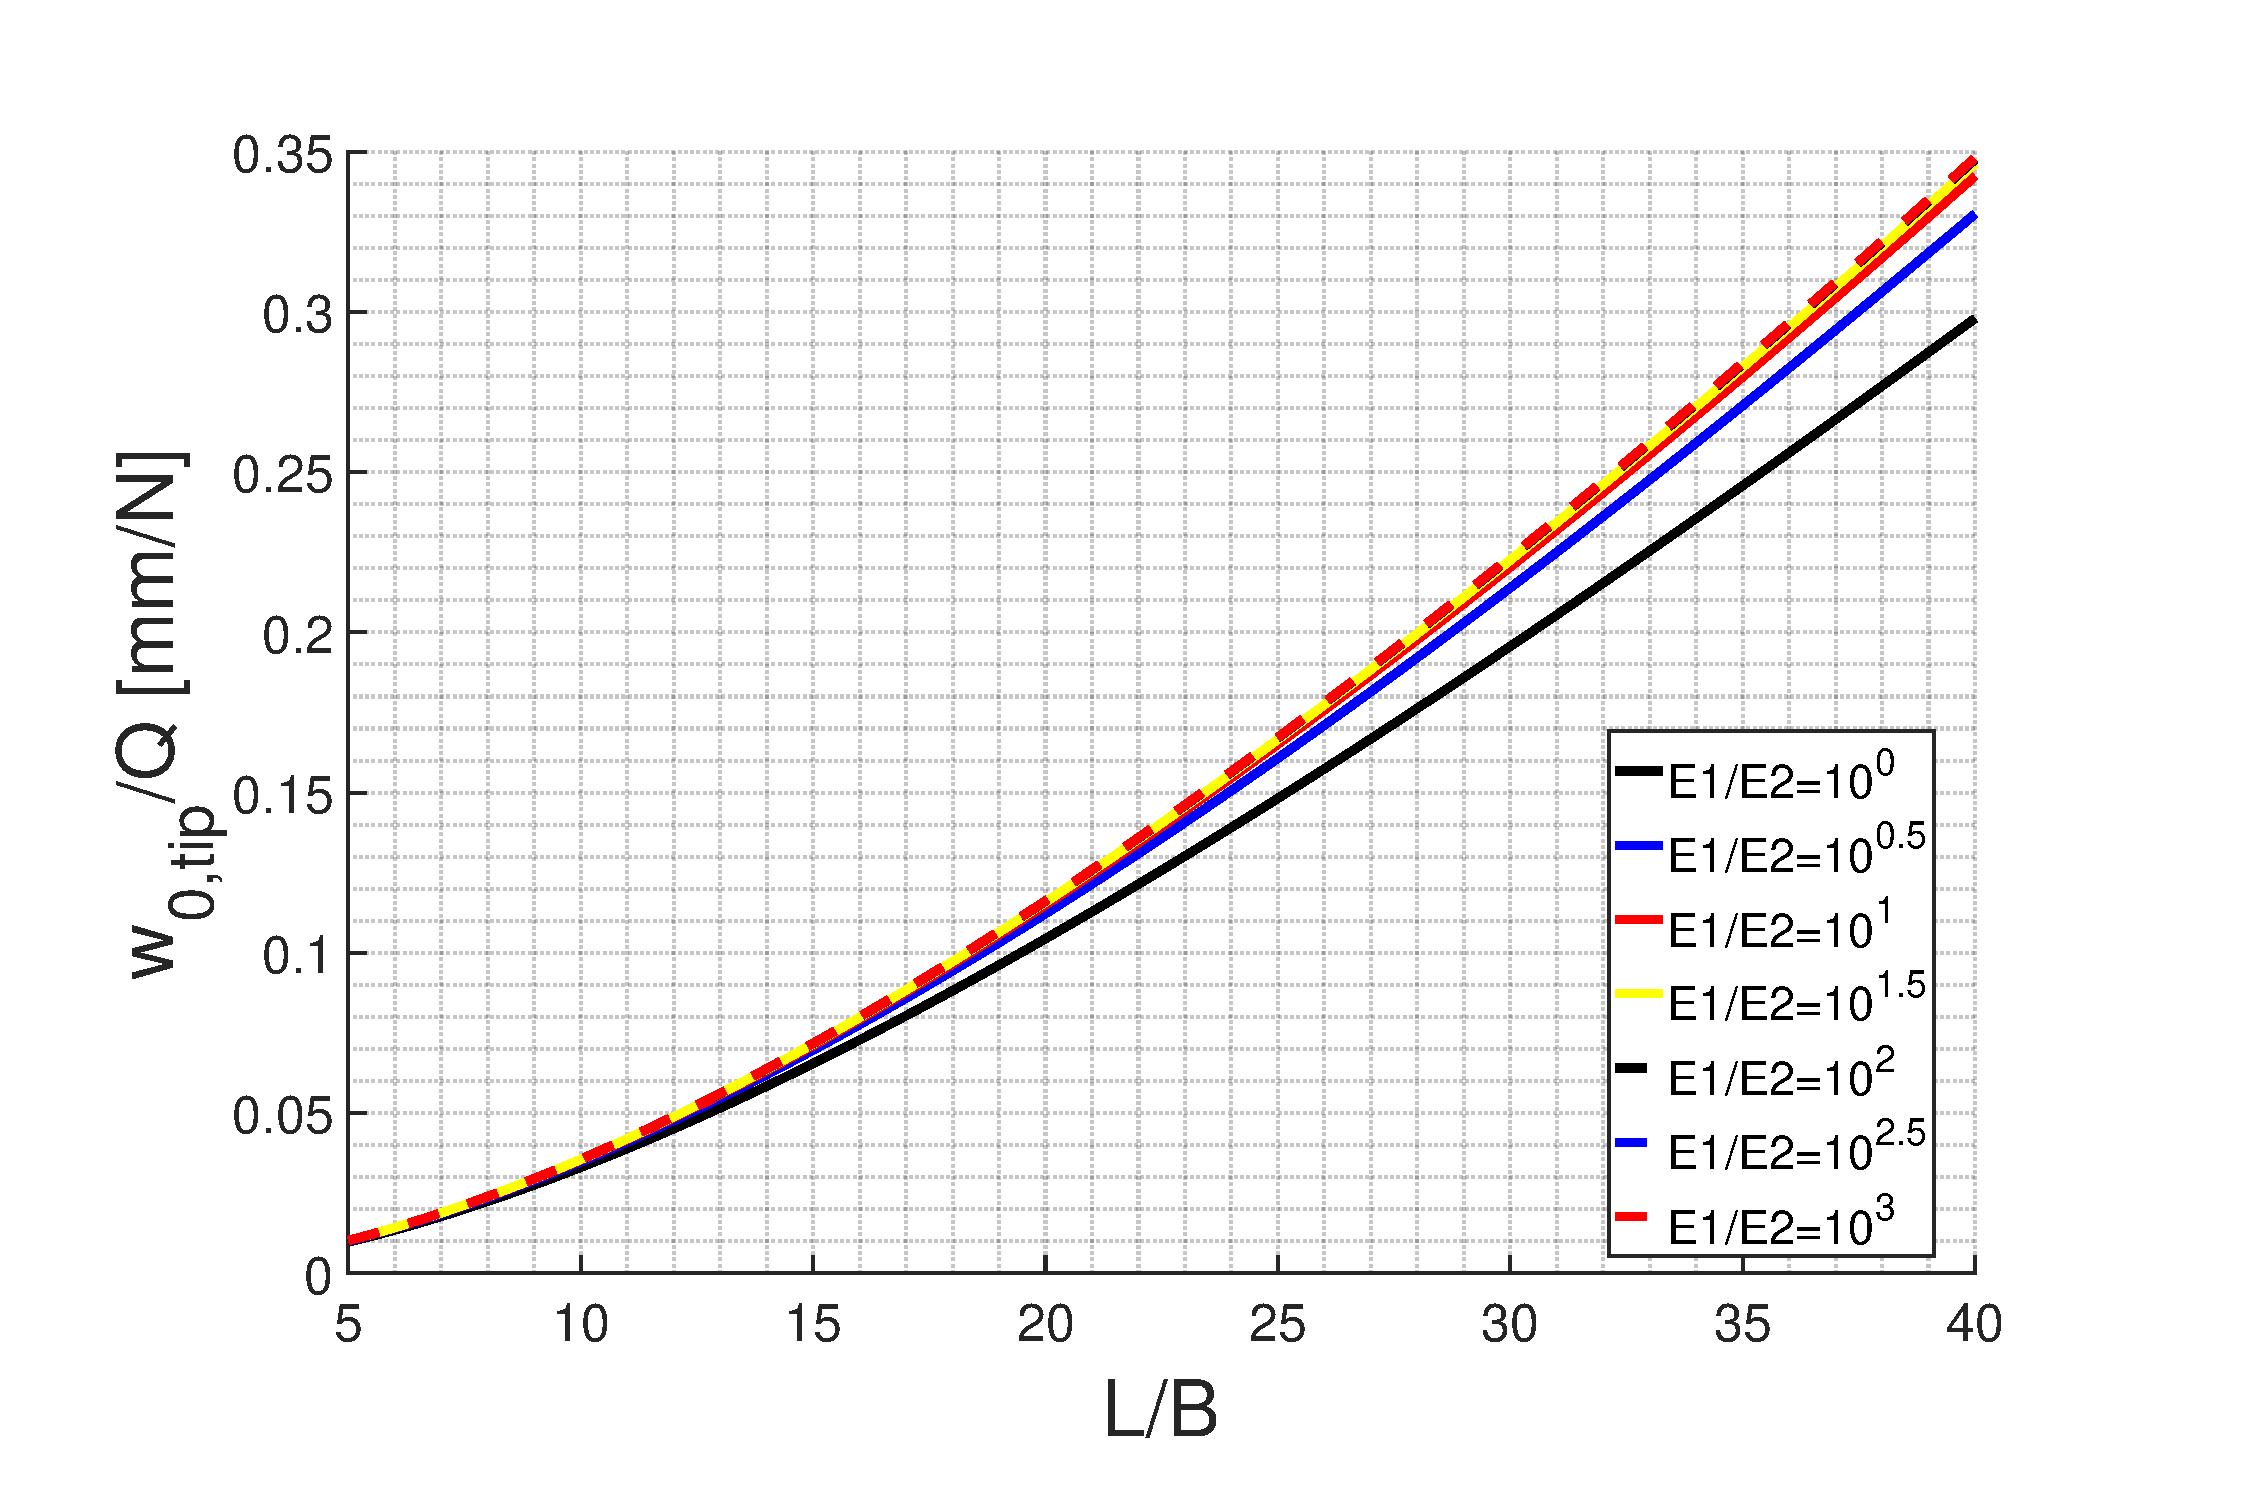
\includegraphics[width=0.8 \textwidth]{../../analytical/figures/woverQ-E1overE2-LoverB}
  \caption[Influence of the slenderness ratio $L/B$ on the deflection compliance]{Influence of the slenderness ratio $L/B$ on the deflection compliance $w_{\mathrm{0,tip}} / Q$ is shown for various values of the stiffness ratio $E_1/E_2$ ranging from $10^0$ to $10^3$. }\label{fig:woverQ-E1overE2-LoverB}
\end{figure}

\begin{figure}[!htpb] %\phi_tip / Q versus L/B, torsional compliance
  \centering
  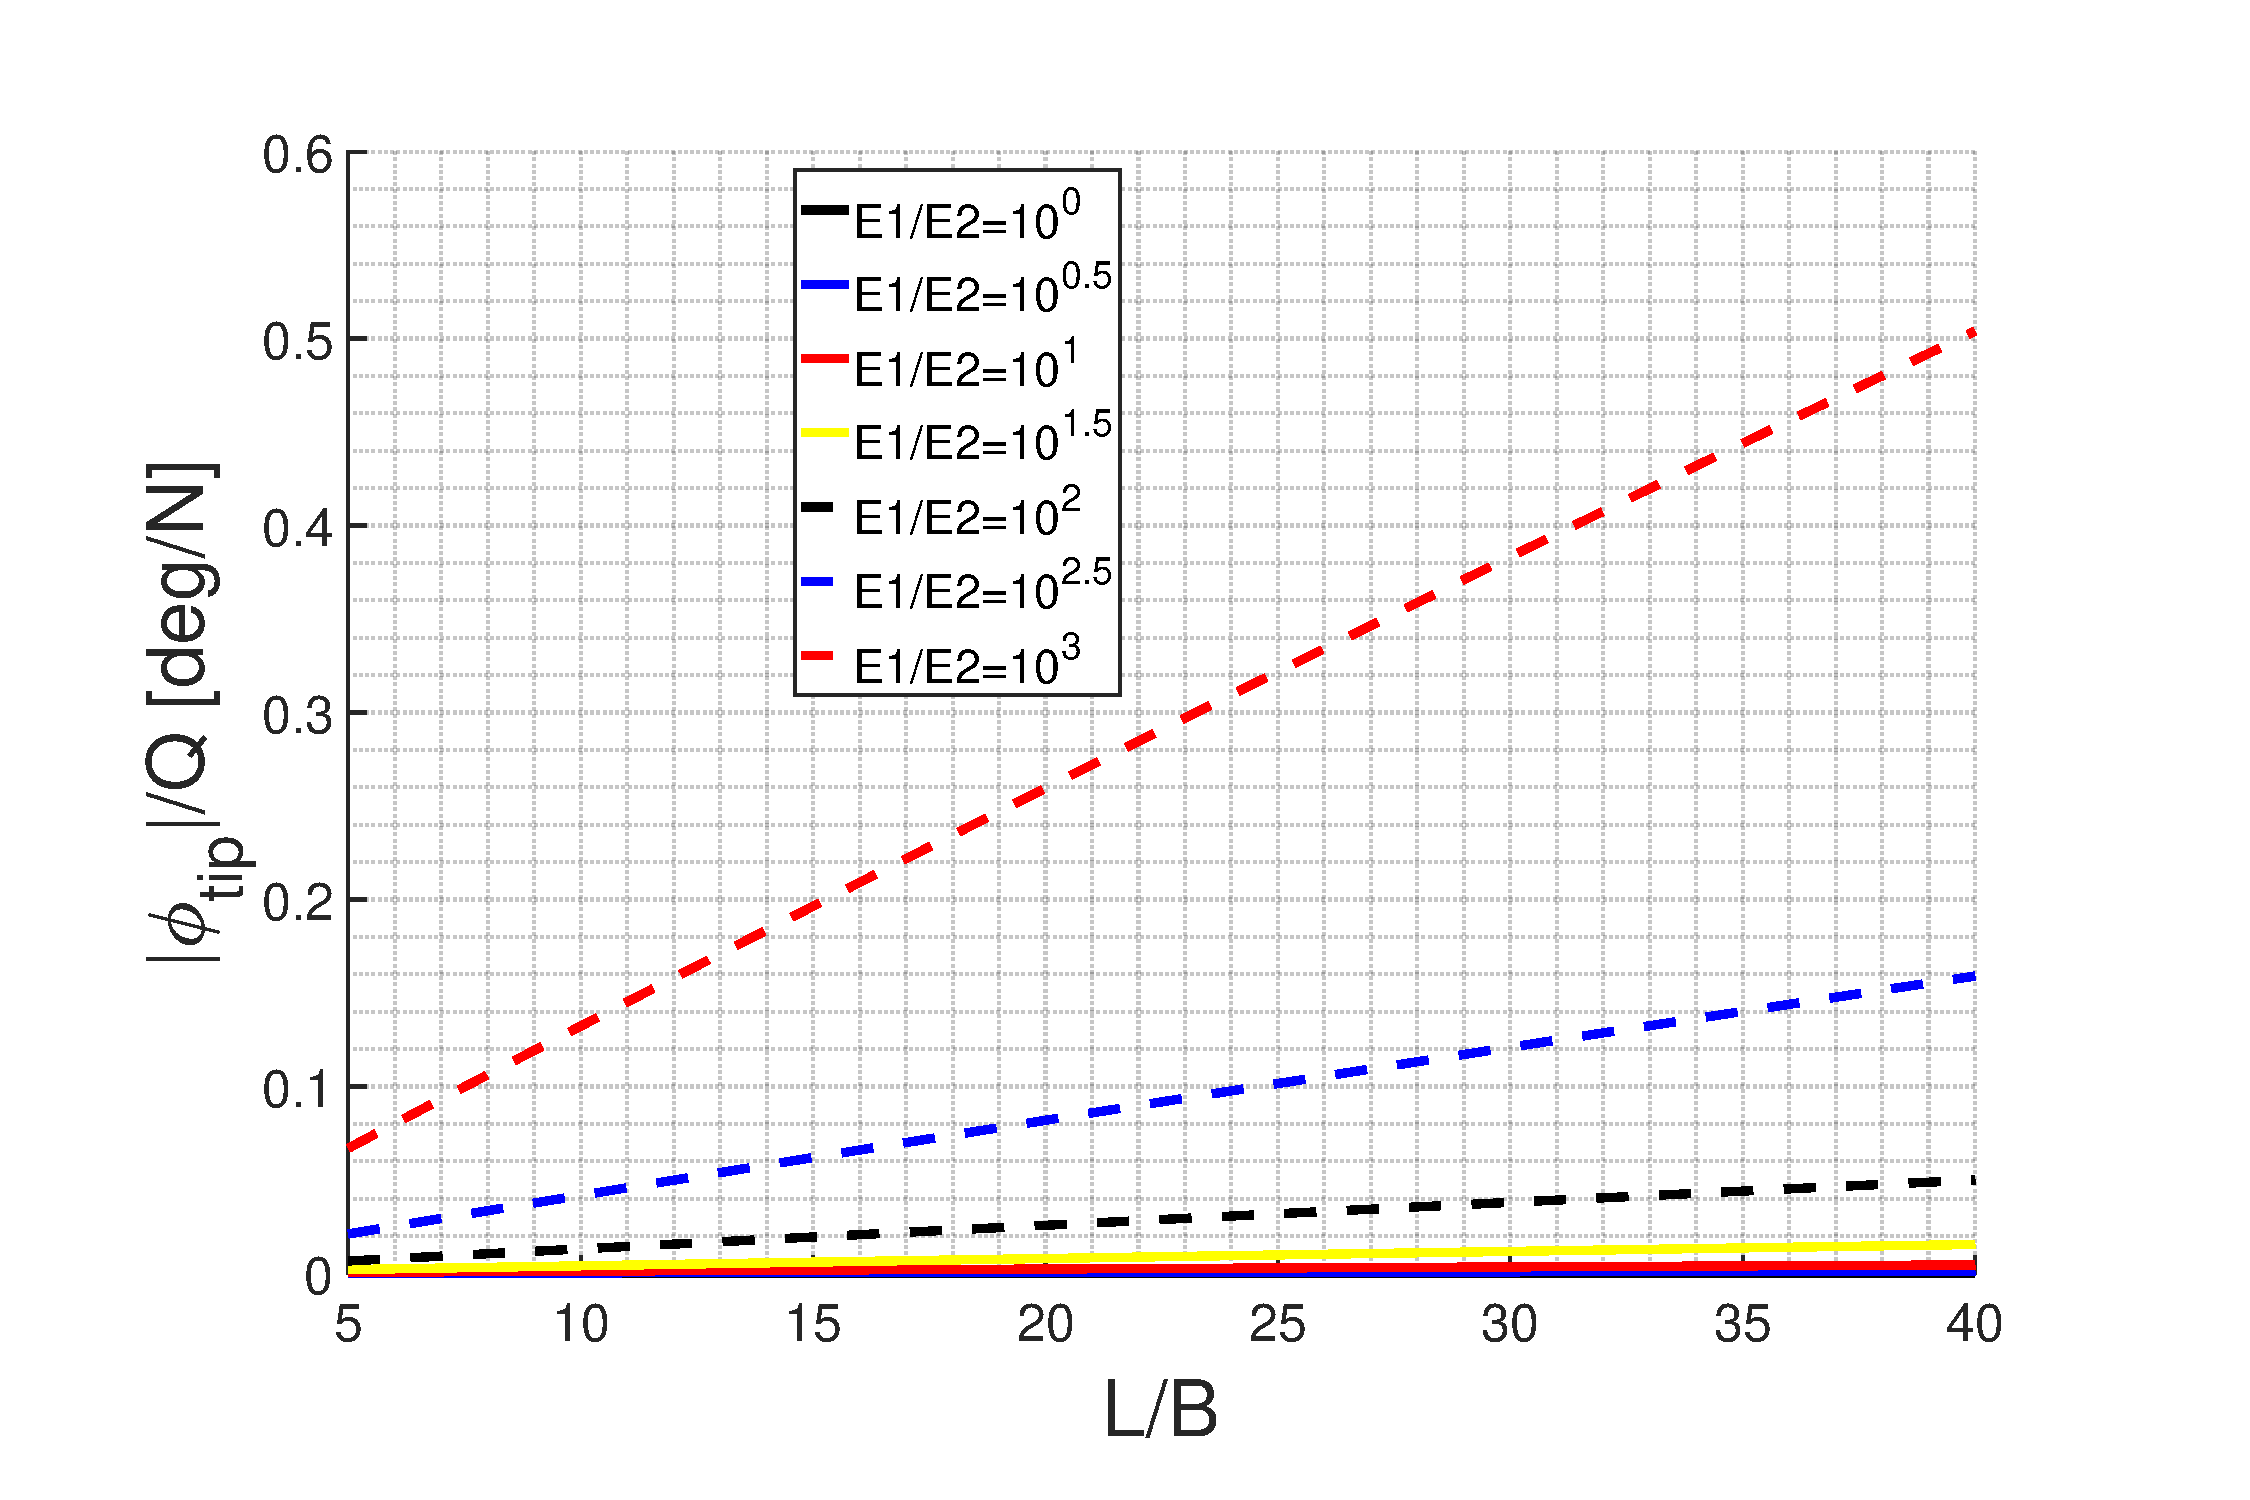
\includegraphics[width=0.8 \textwidth]{../../analytical/figures/phioverQ-E1overE2-LoverB}
  \caption[Influence of the slenderness ratio $L/B$ on the torsional compliance]{Influence of the slenderness ratio $L/B$ on the torsional compliance $|\phi_{\mathrm{tip}}| / Q$ is shown for various values of the stiffness ratio $E_1/E_2$ ranging from $10^0$ to $10^3$. }\label{fig:phioverQ-E1overE2-LoverB}
\end{figure}

\clearpage
\subsubsection{Discussion of the results} \label{subsubsec:disc_results_parametricStudy}

The maximum torsional stiffness $G I_t$ as a function on the cross-sectional aspect ratio $B/H$ can be visualized in Figure \ref{fig:GIt-E1overE2-BoverH}. It can be seen that it appears for $B/H = 1$ when $E_1/E_2 = 1$. Therefore, as it is also shown in \cite{Raither2013a}, the closer the torsional stiffness to the doubly symmetric case, the higher its torsional stiffness. However, when $E_1/E_2 > 10$, the maximum torsional stiffness is shown to appear for $B/H > 1$. A similar conclusion can be extract when analysing the Figure \ref{fig:GIt-E1overE2-t2overt1}, that shows the influence of the thickness ratio $t_2/t_1$ on the torsional stiffness $G I_t$.

In Figure \ref{fig:SC-E1overE2-BoverH} it can be seen that for values $E_2 \ll E_1$, the shear centre position $y_{\mathrm{SC}}$ is approximately constant for $B/H$ variations. In this context, the beam approximates its behavior as if it has an open profile section. However, as the value of $E_1/E_2$ decreases, the influence of the ratio $B/H$ increases showing a bigger influence of the web where the Young's modulus $E_2$ applies. On the other hand, Figure \ref{fig:SC-E1overE2-t2overt1} shows that the bigger the thickness ratio $t_2/t_1$ is, the closer that the shear centre $y_{\mathrm{SC}}$ will be to the vertical axis of simmetry. However, for $E_2 \ll E_1$ the influence of the thickness ratio $t_2/t_1$ is reduced.

The influence of the cross-sectional aspect ratio $B/H$ and the tickness ratio $t_2/t_1$ on the flexural stiffness $E I_y$ is shown to be bigger that that of the Young's modulus ratio $E_1/E_2$, as shown on Figures \ref{fig:EIy-E1overE2-BoverH} and \ref{fig:EIy-E1overE2-t2overt1}, respectively.

% The beam torsional compliance is highly dependant on that torsional moment applied on the beam, that depends on the shear centre $y_{\mathrm{SC}} position. Therefore, as shown on Figure \ref{fig:phioverQ-E1overE2-t2overt1}, the beam's torsional compliance is approximately constant for values of thickness ratio $t_2/t_1 > 1$.


%Comparison of the torsional compliance at the tip against stiffness ratio